\section{Experiments}

In this section, we experimentally evaluate the performance of database engines
generated by \compiler. \compiler is implemented in approximately 9,000 lines of
OCaml code, and as we see in this section, in addition to being able to produce
C++ code for fully recursively compiled queries, it can also produce code for
partially compiled queries to a user-specified nesting level, with the remaining
portions of the query compiled as a relational query plan. Note that a standard
query plan corresponds to zero levels of compilation, while view maintenance
corresponds to one level of compilation.
\comment{
Furthermore, in our query plan
compilation, we do not have a full-fledged query optimizer and joins are
manually selected as indexed nested loops joins or hash joins.
}


\begin{figure}[tb]
\vspace{-6mm}
\hspace{-3mm}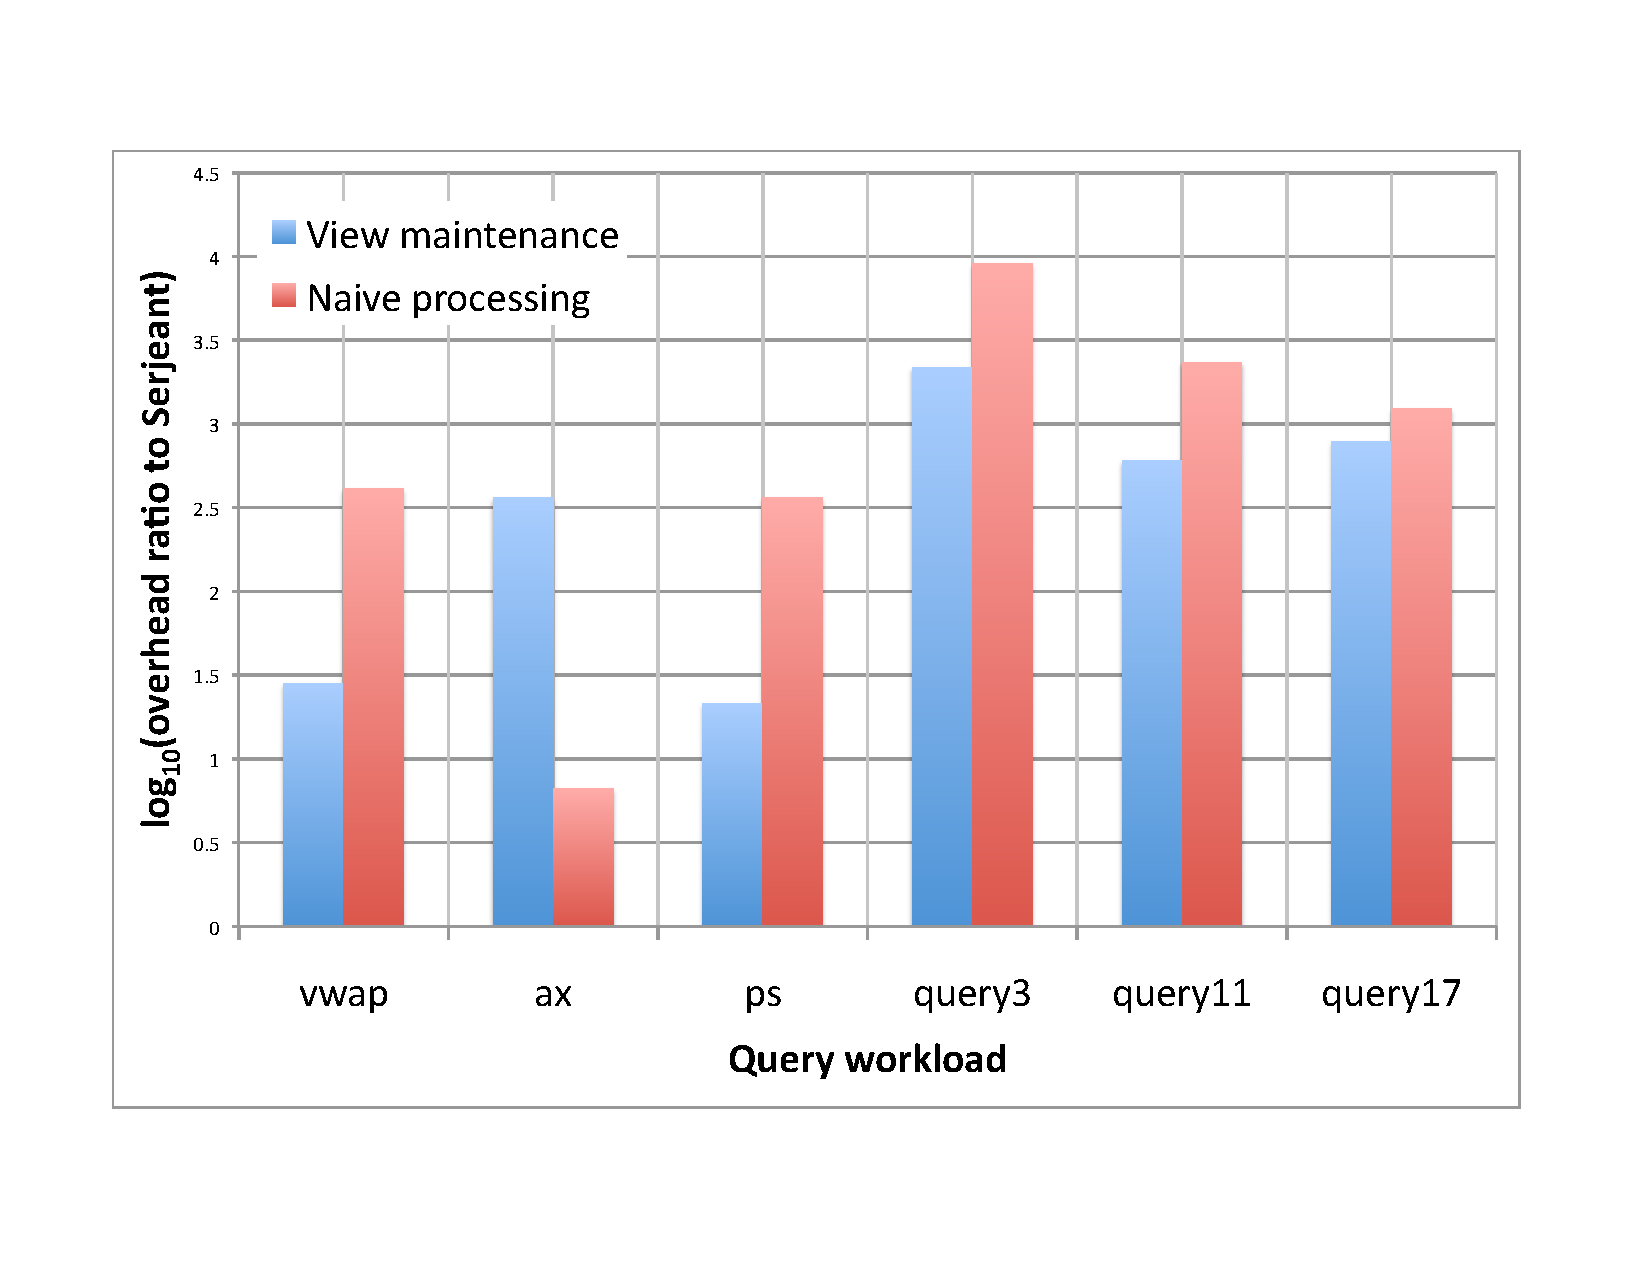
\includegraphics[scale=0.33]{figures/cpu-comparison}
\vspace{-13mm}
\caption{Query processing performance ratio of view maintenance and naive plans
  w.r.t to recursively compiled queries. Note the logarithmic scale y-axis
  indicates the $\log_{10}$ of \compiler's speedup, hence a value of 1
  corresponds to 10x  slower.}
\label{fig:cpucomp}
\end{figure}

\subsection{Experimental setup}
The hardware platform used for our experiments is an 8-core Dual Intel Xeon
2.0Ghz 5335 machine, with 16Gb RAM, running Red Hat Enterprise Linux 5 (Linux
Kernel 2.6.18). Note that the database engines produced by \compiler\ do not
currently exploit query parallelism, and are restricted to executing on a single
core. The underlying C++ compiler was \texttt{g++} v.4.4.0, with compilations
performed with the '-O3' flag alone for optimization.

\feature{Query and data workloads}
Our first workload reflects an automated trading application, where queries are
exemplified by the VWAP query discussed throughout this paper.  The dataset used
for this application is the TotalView-ITCH~\cite{totalview-url} historical order
book from the NASDAQ stock exchange for a 3-month period from December 2008 to
February 2009, for the MSFT (Microsoft) symbol. In addition to the VWAP query,
we consider two other queries, shown in Figure~\ref{fig:obqueries}.
\comment{
The first, denoted Ax, is a query which
determines any simultaneous positioning by a broker on both the bid and asks
orderbooks with a significant difference in order volume. This is commonly
performed by a market maker, or 'ax', to entice buyers or sellers into the
market. The second, denoted PS, tracks the price spread between the bids and
asks orderbooks and is used as an estimate of the trade price. The queries are
shown in Figure~\ref{fig:obqueries}.
}

\begin{figure}[htbp]
Ax finder (Ax) query:
\begin{Verbatim}
select b.broker_id, sum(a.v+-1*b.v)
from bids b, asks a
where b.broker_id = a.broker_id
and ((a.p > 1000+b.p) or (b.p > 1000+a.p))
group by b.broker_id
\end{Verbatim}
Price spread (PS) query:
\begin{Verbatim}
select sum(a.p+-1*b.p) from bids b, asks a
where (b.v>0.0001*(select sum(b1.v) from bids b1))
and (a.v>0.0001*(select sum(a1.v) from asks a1))
\end{Verbatim}
\vspace{-3mm}
\caption{Orderbook queries: Ax and PS.}
\label{fig:obqueries}
\end{figure}

Our second workload reflects the online data warehousing application discussed
in the introduction. Here the dataset is TPC-H, generated with scale factor 1
for in-memory processing. The queries used here are queries 3, 11 and 17 --
\comment{
which respectively determine shipping priorities (i.e. finding unshipped orders with
high value), important stocks for suppliers in various nations, and the revenue
obtained from small quantity orders.
}
we refer to the TPC-H specification~\cite{tpch-url} for their details.

\subsection{Query Processing Performance}
Our first set of experimental results look at the query processing performance
of three \compiler-generated engines, namely fully recursively compiled queries,
view maintenance queries, and standard query plans (we refer to these as
\textit{naive} plans since they do not attempt to perform any incremental
computation). We start with Figure~\ref{fig:cpucomp}, which illustrates the
per-tuple processing overhead of view maintenance queries and naive plans with
respect to \compiler's performance. To emphasize, these are all query plans
compiled directly to C++ code, and subsequently to machine code, and thus are
already eliminating the overhead involved in interpreting query plans as is done
in System-R style database systems.

Figure~\ref{fig:cpucomp} shows the significant performance gains attained by
applying recursive compilation across all queries, outperforming both view
maintenance and naive compilation by a range of 1-4 orders of magnitude (that is
10x-10000x factor improvement). Other trends shown in this figure include that
with the exception of the Ax query, view maintenance tends to outperform naive
processing, as to be expected, due to the slightly simpler nature of the query
following one delta transformation pass. However, as one of the primary
conjectures of this paper, these results show that view maintenance does not go
far enough -- \compiler\ significantly outperforms view maintenance queries in
our entire workload.


\begin{figure}[htbp]
\begin{center}
\begin{tabular}{|r|c|c|c|}
\hline
      & \multicolumn{3}{|c|}{Query processing times (secs)}\\
Query & \compiler & VM & Naive\\
\hline
vwap     & 0.00015     & 0.0042   & 0.0619 \\
ax       & 0.000614    & 0.2235   & 0.0041 \\
ps       & 0.000792    & 0.0170   & 0.2881 \\
query3   & 7.41E-06    & 0.0162   & 0.0675 \\ 
query11  & 3.49E-05    & 0.0210   & 0.0818 \\
query17  & 3.66E-05    & 0.0287   & 0.0454 \\
\hline
\end{tabular}
\end{center}
\vspace{-3mm}
\caption{Per-tuple processing times for the recursive compilation, view
  maintenance and naive query processing strategies.}
\label{tbl:cpuabs}
\end{figure}


The figure also reveals a significant speedup gap for \compiler between the
orderbook queries and the TPC-H queries, where \compiler tends to be
approximately 3 orders of magnitude faster for TPC-H queries and approximately
1-25 orders of magnitude faster for orderbook queries. This can be explained by
the different dataset characteristics -- order books remain relatively small
during the run, thus the effects of performing fully incremental processing are
relatively diminished compared to the TPC-H case. We expect our technique to
provide maximal advantages as the in-memory database size approaches that of
main-memory capacities.
We now briefly discuss the results of the Ax query. The
Ax query is a binary join query with simple range predicates, and a group-by
aggregate. In this scenario, our naive implementation uses a nested-loops join
that can be highly optimized by the C++ compiler for efficient register and
cache usage, as opposed to an indexed nested-loops join which uses map data
structures. We plan on investigating the cache performance of \compiler's
queries as a topic of future work.


\begin{figure}[htbp]
\vspace{-9mm}
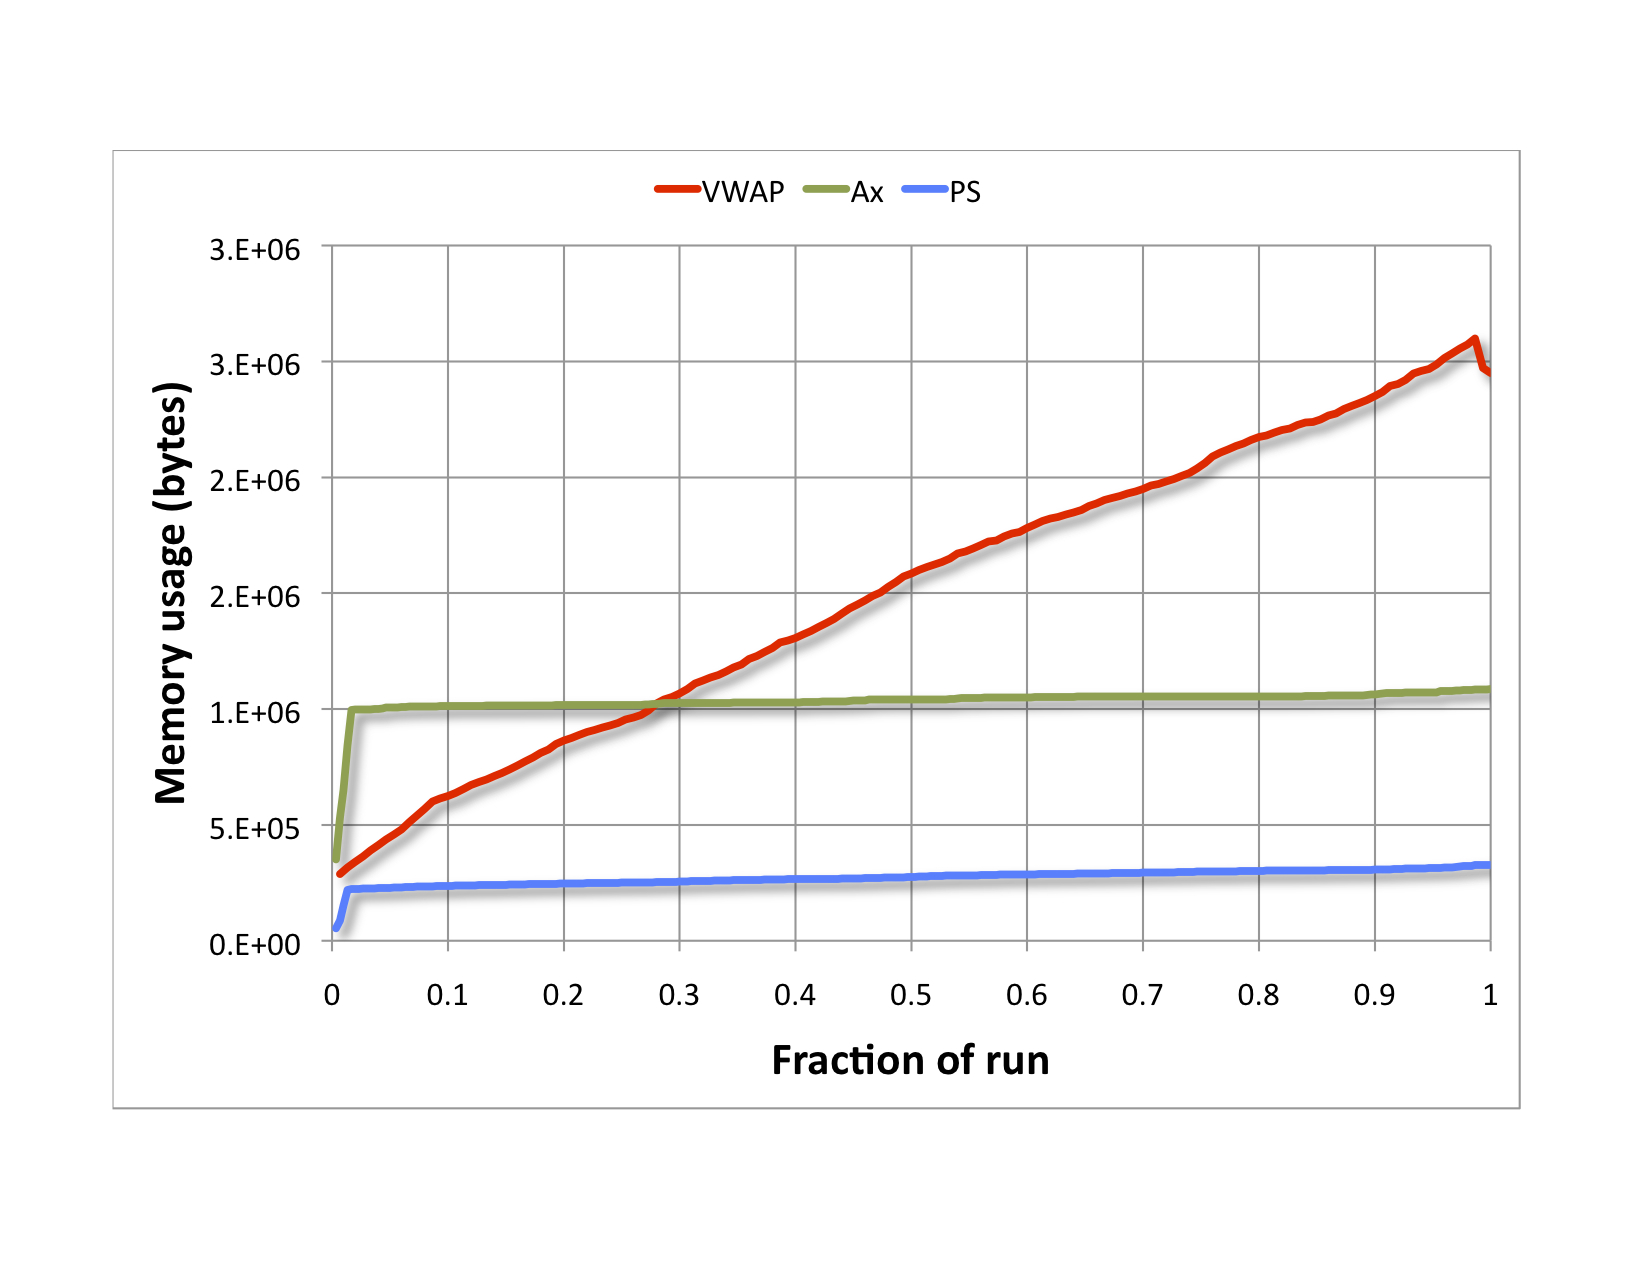
\includegraphics[scale=0.31]{figures/orderbk-mem}
\vspace{-14mm}
\caption{Memory utilization of \compiler's datastructures for the VWAP, Ax and
  PS queries}
\label{fig:orderbkmem}
\end{figure}

Finally, since our figure only indicates relative performances, we present
absolute per-tuple processing times in Table~\ref{tbl:cpuabs}. This reaffirms
that \compiler\ is also efficient in absolute terms, with the TPC-h per-tuple
processing times on the order of microseconds and 10s of microseconds.
\comment{
While our experiments were performed in batch fashion and thus indicate
throughput, these low per-tuple overheads give us confidence that our engines
are also capable of providing low latencies.
}

\subsection{Memory Utilization}
The next set of memory results looks at the memory utilization of \compiler's
internally maintained maps. These are displayed separately for the orderbook
queries and the TPC-H queries in Figure~\ref{fig:orderbkmem} and
Figure~\ref{fig:tpchmem} respectively. We start with Figure~\ref{fig:orderbkmem}
which concerns the VWAP, Ax, and PS queries.


The first point we make is to reaffirm the point that order books are small (but
frequently and arbitrarily updated), and this can be seen by the scale of the
y-axis in the figure -- total memory consumption is on the order of a few
megabytes. Next we see that both the Ax and PS queries tail off in their memory
consumption very early on in their runs. The internal datastructures kept for PS
are minimal since there are no group-bys nor is there any nested variable usage
in the query. For the Ax query, memory utilization is slightly larger due to the
group-by on broker ids, as well as the join predicate on the price attribute
(which results in a loop variable).
\comment{
Thus one of the maps maintained internally
by \compiler\ uses both of these attributes as keys, and given that the price
attribute is a numeric type, this map dominates memory usage. Note that despite
price being a double precision type, order book prices do not take on
arbitrarily many values, rather are typically given in increments of 100 units
according to the NASDAQ ITCH specification.
}

\begin{figure}[htbp]
\vspace{-9mm}
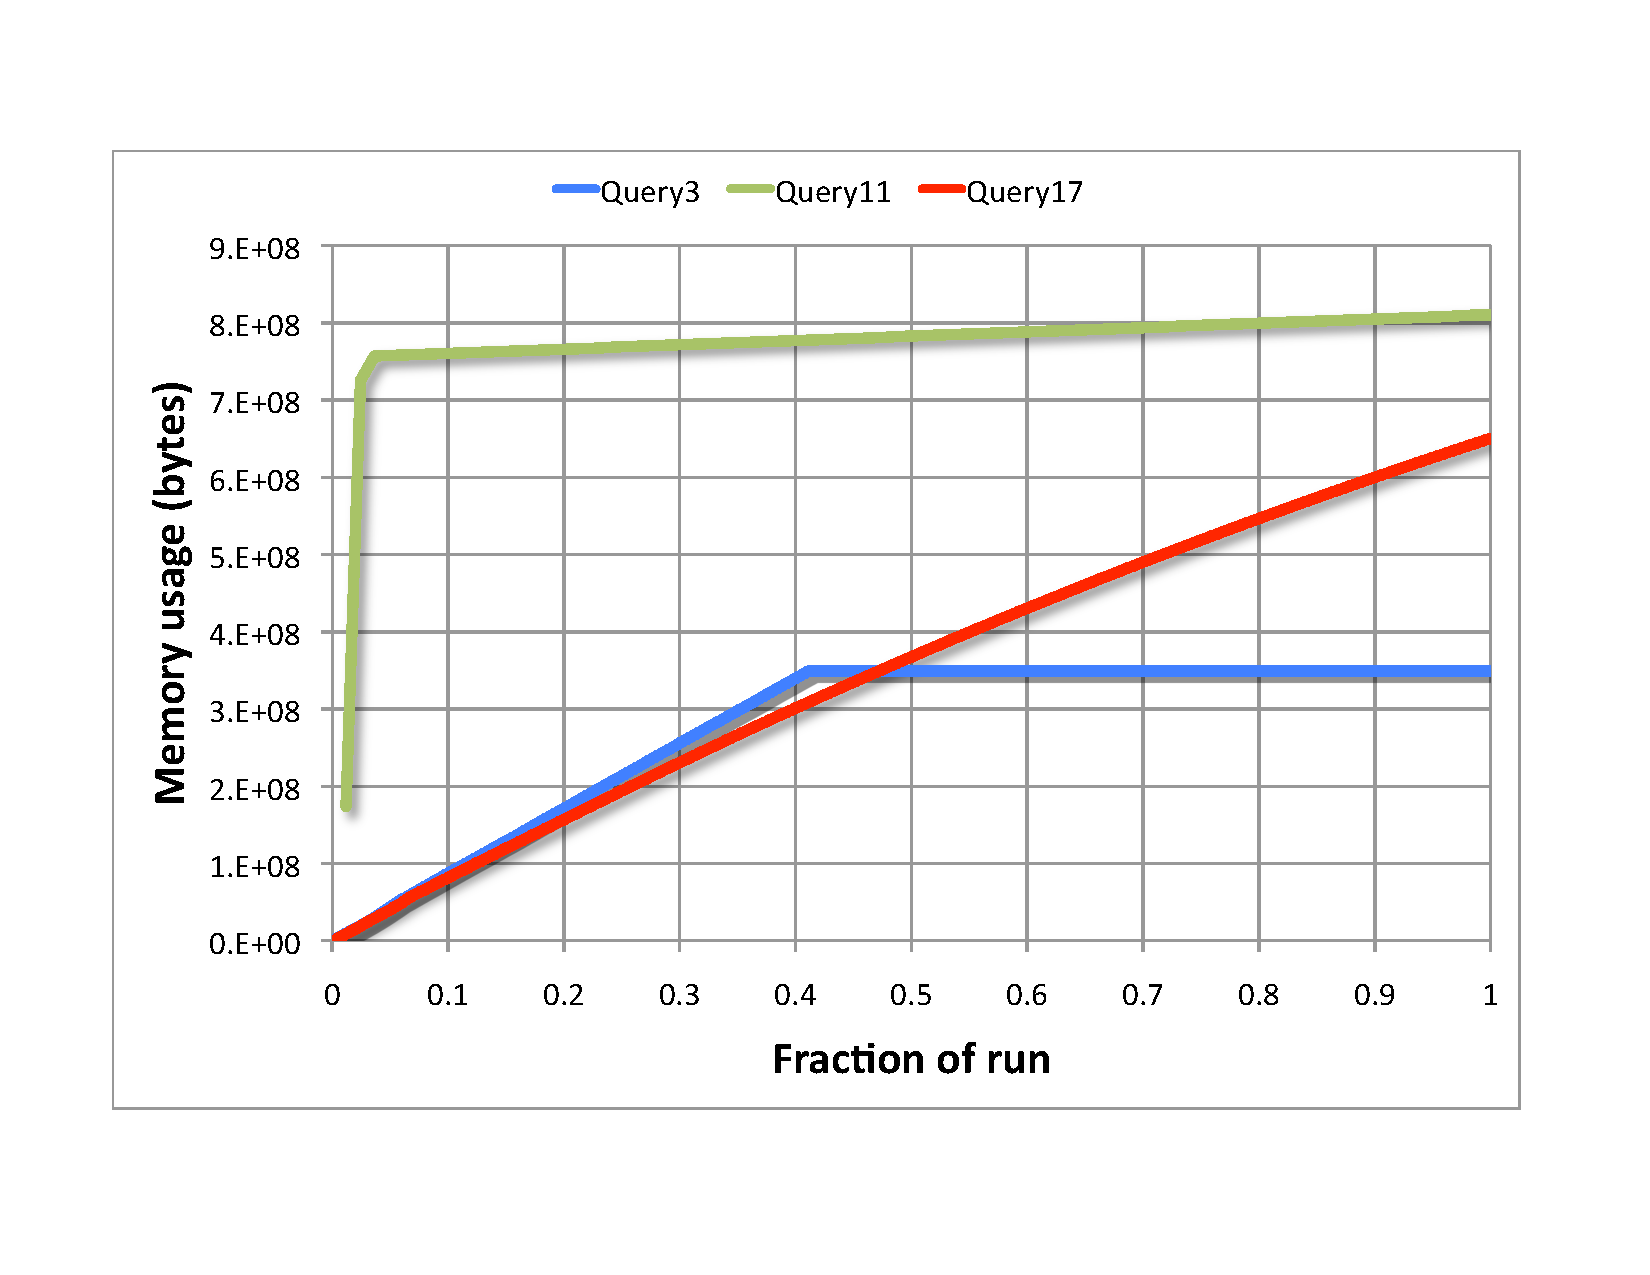
\includegraphics[scale=0.31]{figures/tpch-mem}
\vspace{-14mm}
\caption{Memory utilization of \compiler's datastructures for TPC-H query 3, 11
  and 17.}
\label{fig:tpchmem}
\end{figure}

The VWAP query has the largest memory consumption due to the presence of a
nested variable usage, namely the price attribute. This nested variable usage
requires us to keep a map for a subquery, parameterized by this variable, and
furthermore, to correctly handle deletions and reclaim map keys, we maintain the
bids relation itself for the VWAP query. It is the full bids relation which
dominates memory usage in the VWAP query, but again, since orderbooks are
small, this does not consume significant space. Alternatively, to avoid keeping
the bids relation, we could simply maintain the map for every domain value
seen. However this incurs additional computational overhead for inactive domain
values, but this decision could be left to an optimizer.

Figure~\ref{fig:tpchmem} demonstrates that the TPC-H queries consume
significantly more memory than the order book queries primarily due to the the
larger domains of map key attributes, and the fact that our application is an
append-only data warehouse. The figure shows that queries 3 and 11 tail off in
their memory utilization during the run, with query 3 consuming approximately
350Mb, and query 11 approximately 800Mb.  The memory consumption of query 3 is
loosely evenly divided between 5 maps. Query 11's memory consumption is however
skewed, with a single map. Query 17 on the other hand scales almost linearly
throughout the experiment run. This query uses 8 datastructures (maps and
domains), with two sizeable maps consuming nearly 600Mb of memory.

\comment{
 The memory consumption of query 3 is
loosely evenly divided between 5 maps, one for the group-by aggregate result,
and the rest as aggregates decomposed over the join of the lineitem, orders and
customers tables. Query 11's memory consumption is however skewed, with a single
map which has both the partkey and supplier key as its index dominating. Query
17 on the other hand scales almost linearly throughout the experiment run. This
query uses 8 datastructures (maps and domains), with two sizeable maps consuming
nearly 600Mb of memory at the end of the run. These maps are both sub-aggregates
over the lineitem relation, with a map key of the partkey attribute,
instantiated by the flattening of the nested aggregate query.
}

\comment{
\begin{figure}[tb]
\begin{tabular}{|r|c|c|c|}
\hline  & \multicolumn{3}{|c|}{Map datastructure}\\
\hline
Query   & Name & Defining term & Memory usage \\
vwap    & & &
\\
ax      & & &
\\
ps      & & &
\\
query3  & & &
\\
query11 & & &
\\
query17 & & &
\\
\hline 
\end{tabular}
\end{figure}

The full details of the maps instantiated for each query and their memory usage
at the end of the experiment can be found in Table~\ref{tbl:map-mem}.
}


\begin{figure}[htbp]
\begin{center}
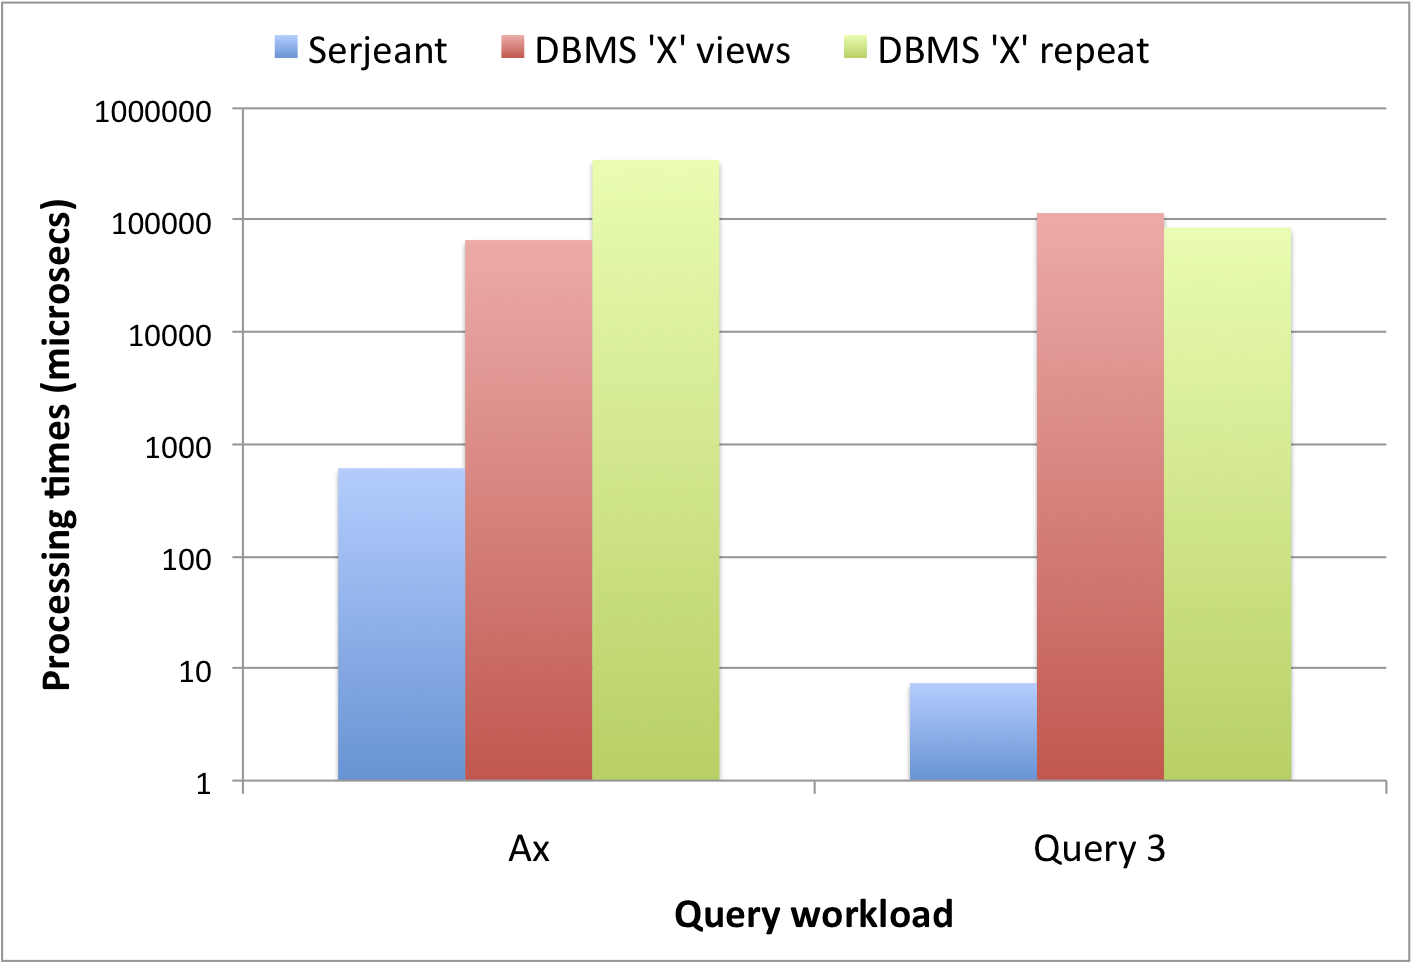
\includegraphics[scale=0.32]{figures/dbcomp}
\end{center}
\vspace{-4mm}
\caption{Comparison of \compiler's processing times to DBMS 'X'.}
\label{fig:dbcomp}
\end{figure}


\subsection{DBMS comparison}
In the final part of our experiments section, we compare the performance of a
commerical DBMS 'X' to \compiler, reporting on the per-tuple processing time for
queries implemented using incremental materialized views, and naive processing
in DBMS 'X'. Note that many commercial database systems are extremely restricted
in the kinds of queries supported via incremental view maintenance, and to the
best of our knowledge, none can handle the general nested aggregate queries
supported by \compiler.
\comment{
We provide the following references to DBMS
documentation on queries that may be maintained incrementally in three major
DBMS:
i) Oracle: {\tiny
    \url{http://download.oracle.com/docs/cd/B28359_01/server.111/b28313/basicmv.htm#i1007007}}
ii) MS SQL Server 2008: {\tiny
    \url{http://msdn.microsoft.com/en-us/library/dd171921.aspx}}
iii) IBM DB2: {\tiny
    \url{http://publib.boulder.ibm.com/infocenter/db2luw/v9r5/index.jsp?topic=/com.ibm.db2.luw.sql.ref.doc/doc/r0000927.html}}.
}


Given these restrictions, we are only able to compare using the Ax and TPC-H
Query 3 workloads. The results are shown in Figure~\ref{fig:dbcomp}, with a
logarithmic scale for the processing times. Note the the repeat method
corresponds to naive query processing, where the original plan-based query is
issued following every update. This figure reiterates the findings of directly
compiling the methods from \compiler. We see that \compiler significantly
outperforms both view maintenance and the naive processing mechanisms by at
least 2 orders of magnitude for the Ax query, and by 4 orders of magnitude on
TPC-H query 3. As expected, incremental view maintenance outperforms naive
processing for the Ax query, however, somewhat surprisingly, the materialized
view implementation of query 3 performs worse than the naive processing
method. We are currently in the process of determining the cause.



%
%
%
%
%
\comment{
\subsection{Query Processing Performance}

\subsubsection{Synthetic workloads}
\begin{itemize}
\item Nested workload: simple linear nesting, with varying nesting levels $k=1..5$ i.e.
\[sum_{sum_{sum_{f}(Q_1)}(Q_2)}(Q_3)\]

\item Join workload: fixed set of join graphs, with varying \# relations
  $k=1..10$. Join graphs should include chains, and stars, and if time permits
  cycles simplified with hypergraph decomposition.

\item What dataset should we use here? TPCH/orderbook data, or generate
  synthetic distributions?

\item Predicted running times:
    \begin{itemize}
    \item Indexed $k$-way nested loops joins w/ accumulators: $O(n\log^{k-1}{n})$
    \item RC(k): $\sum_{m \in maps(k)} {\mbox{update cost}(m)}$
    \end{itemize}
\end{itemize}

\begin{figure}
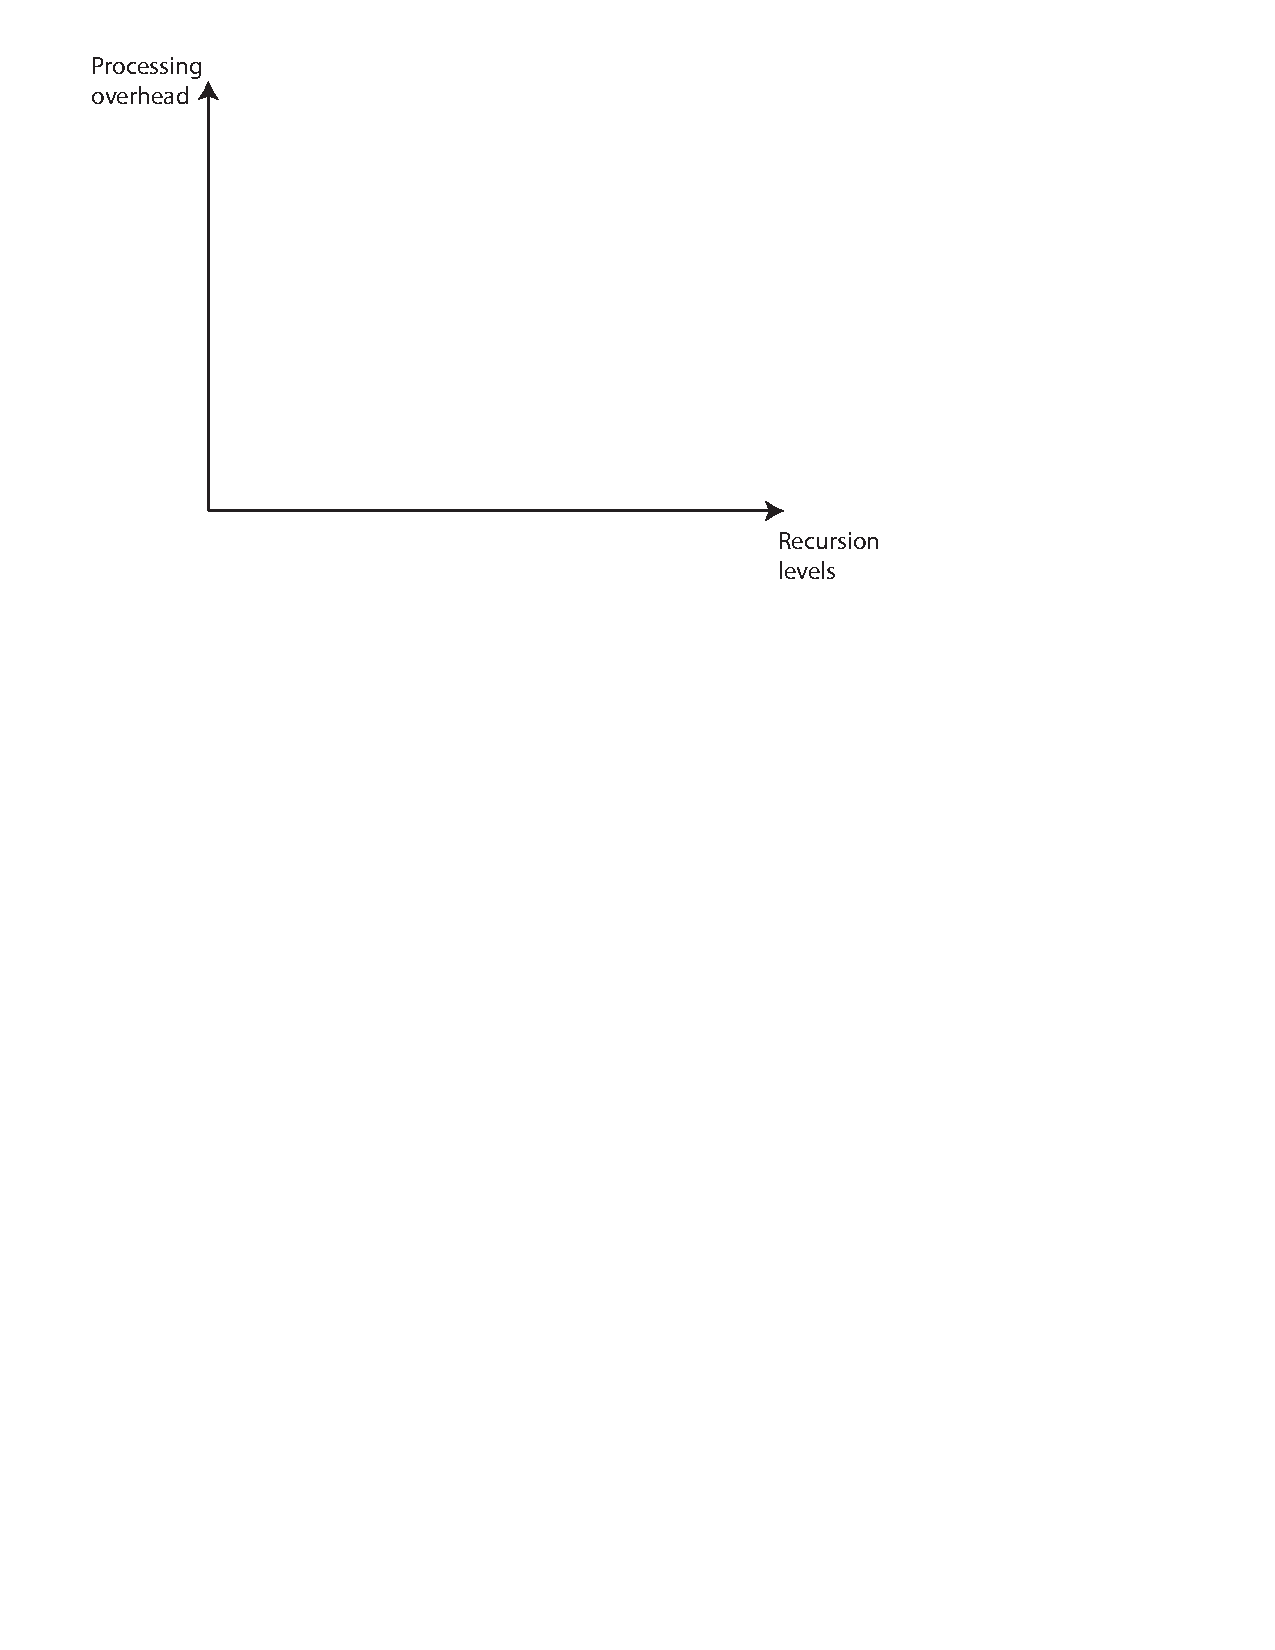
\includegraphics[scale=0.6]{figures/axes-rlevels.pdf}
\caption{Query processing overhead under varying degrees of recursive
compilation aggressiveness, for a \textit{k}-nested query.}
\label{fig:overhead-recursion-levels-nesting}
\end{figure}

\begin{figure}
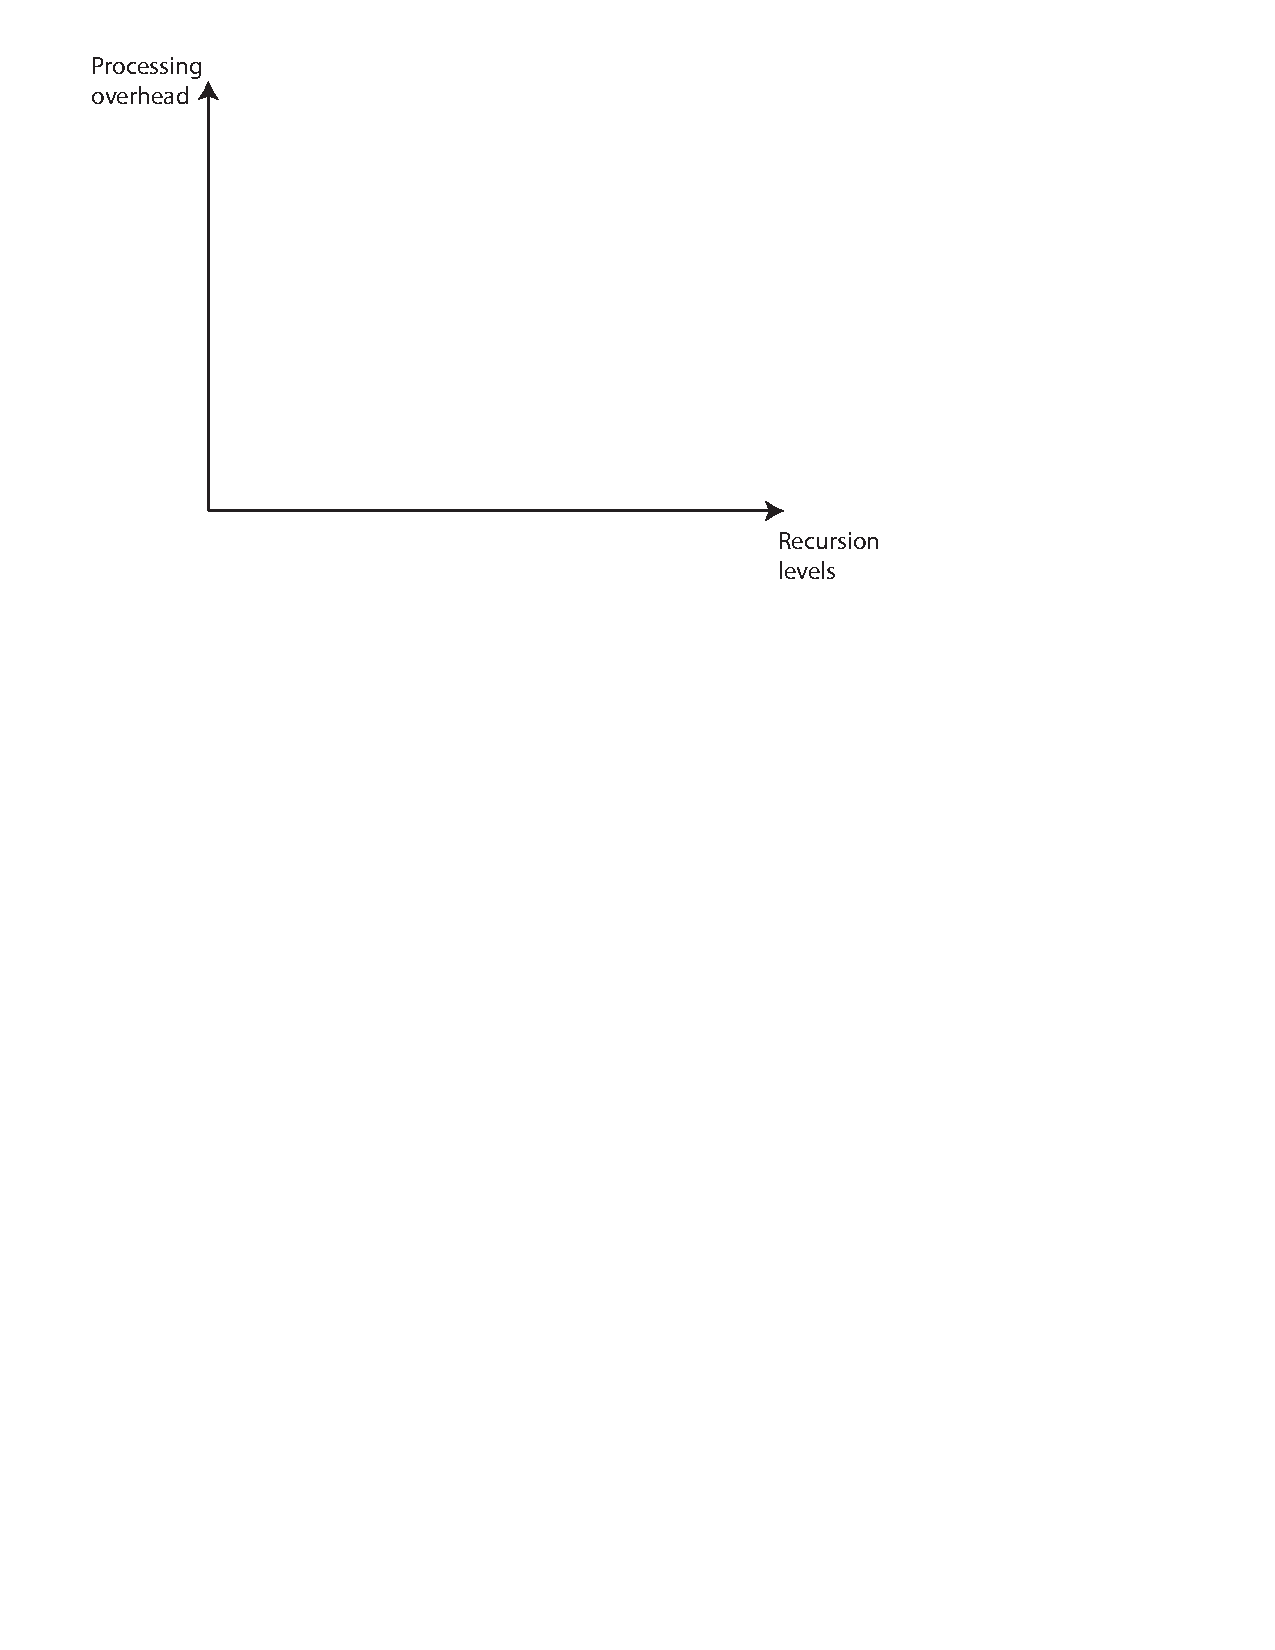
\includegraphics[scale=0.6]{figures/axes-rlevels.pdf}
\caption{Query processing overhead under varying degrees of recursive
compilation aggressiveness, for a \textit{k}-way join.}
\label{fig:overhead-recursion-levels-join}
\end{figure}

\begin{figure}
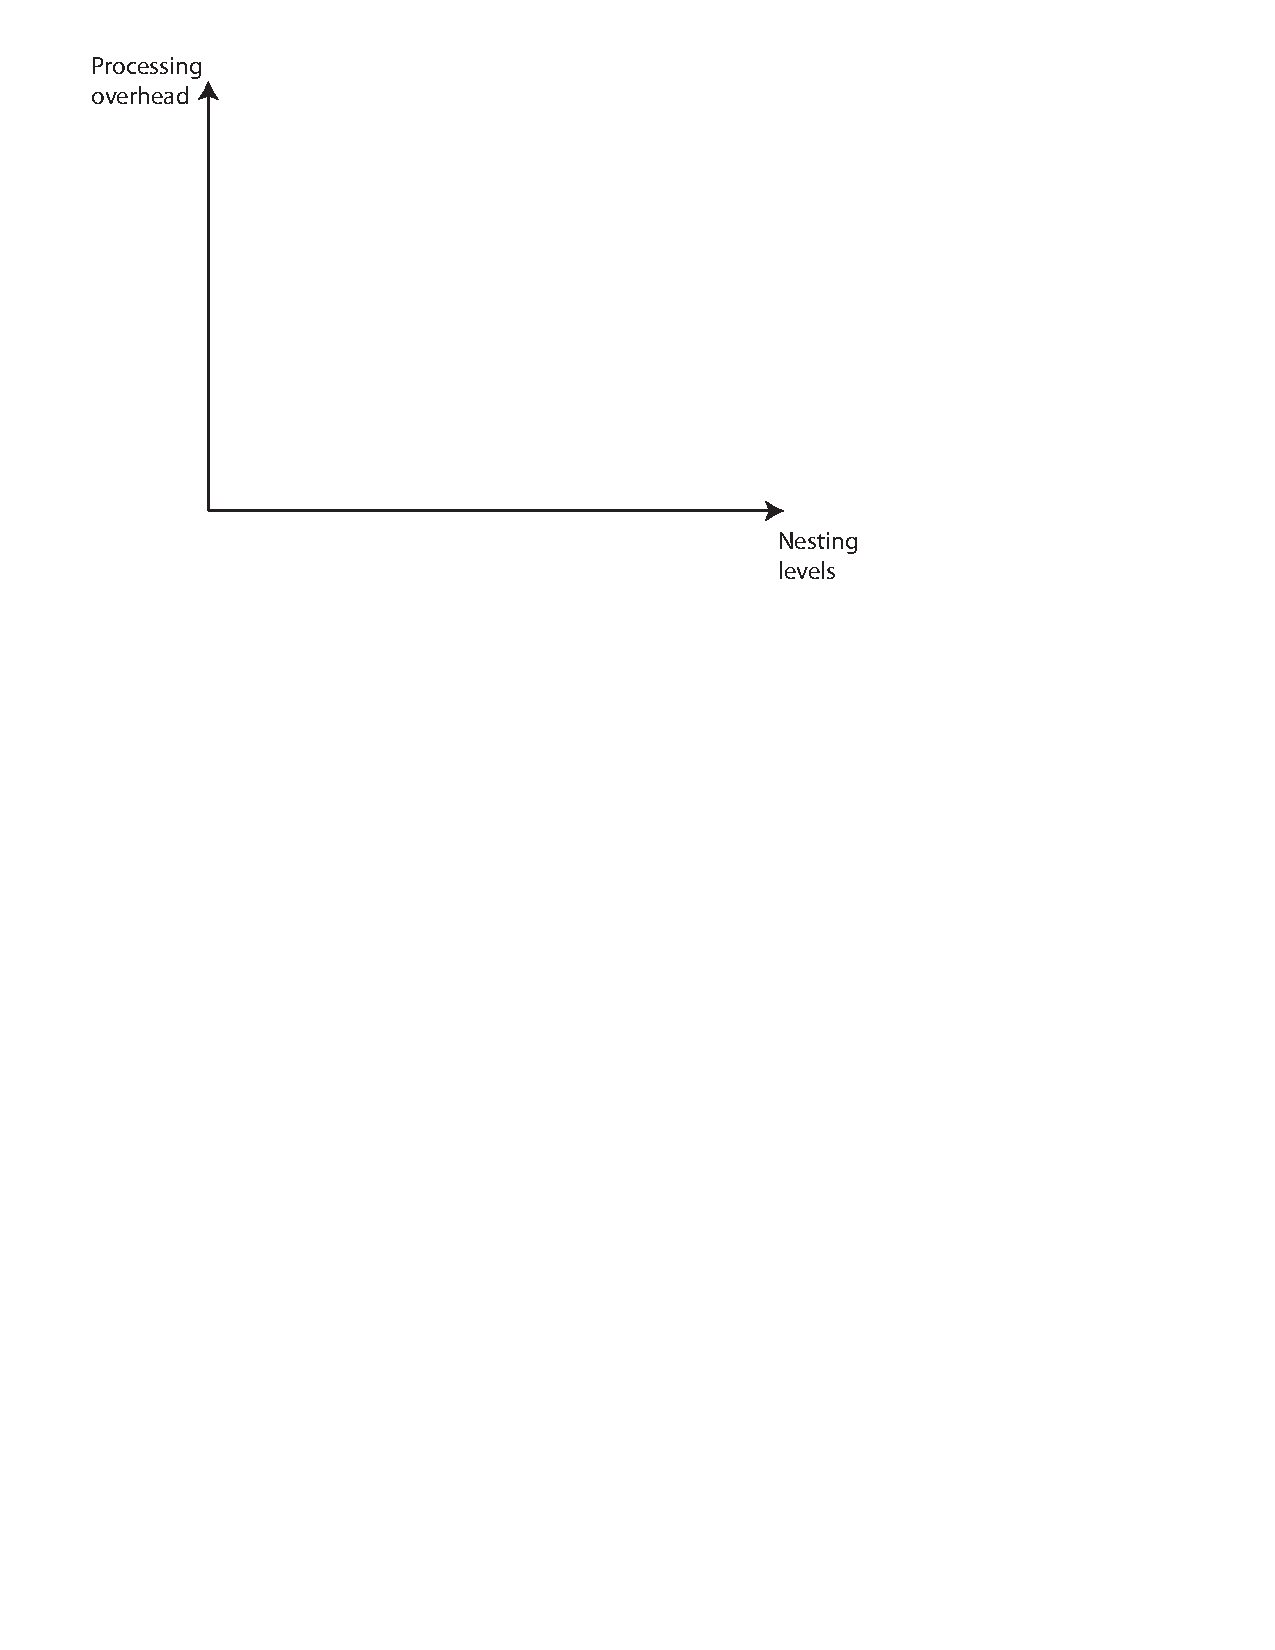
\includegraphics[scale=0.6]{figures/axes-nlevels.pdf}
\caption{Query processing overhead under varying nesting workloads, for
recursive compilation and incremental view maintenance.}
\label{fig:overhead-workload-nesting}
\end{figure}

\begin{figure}
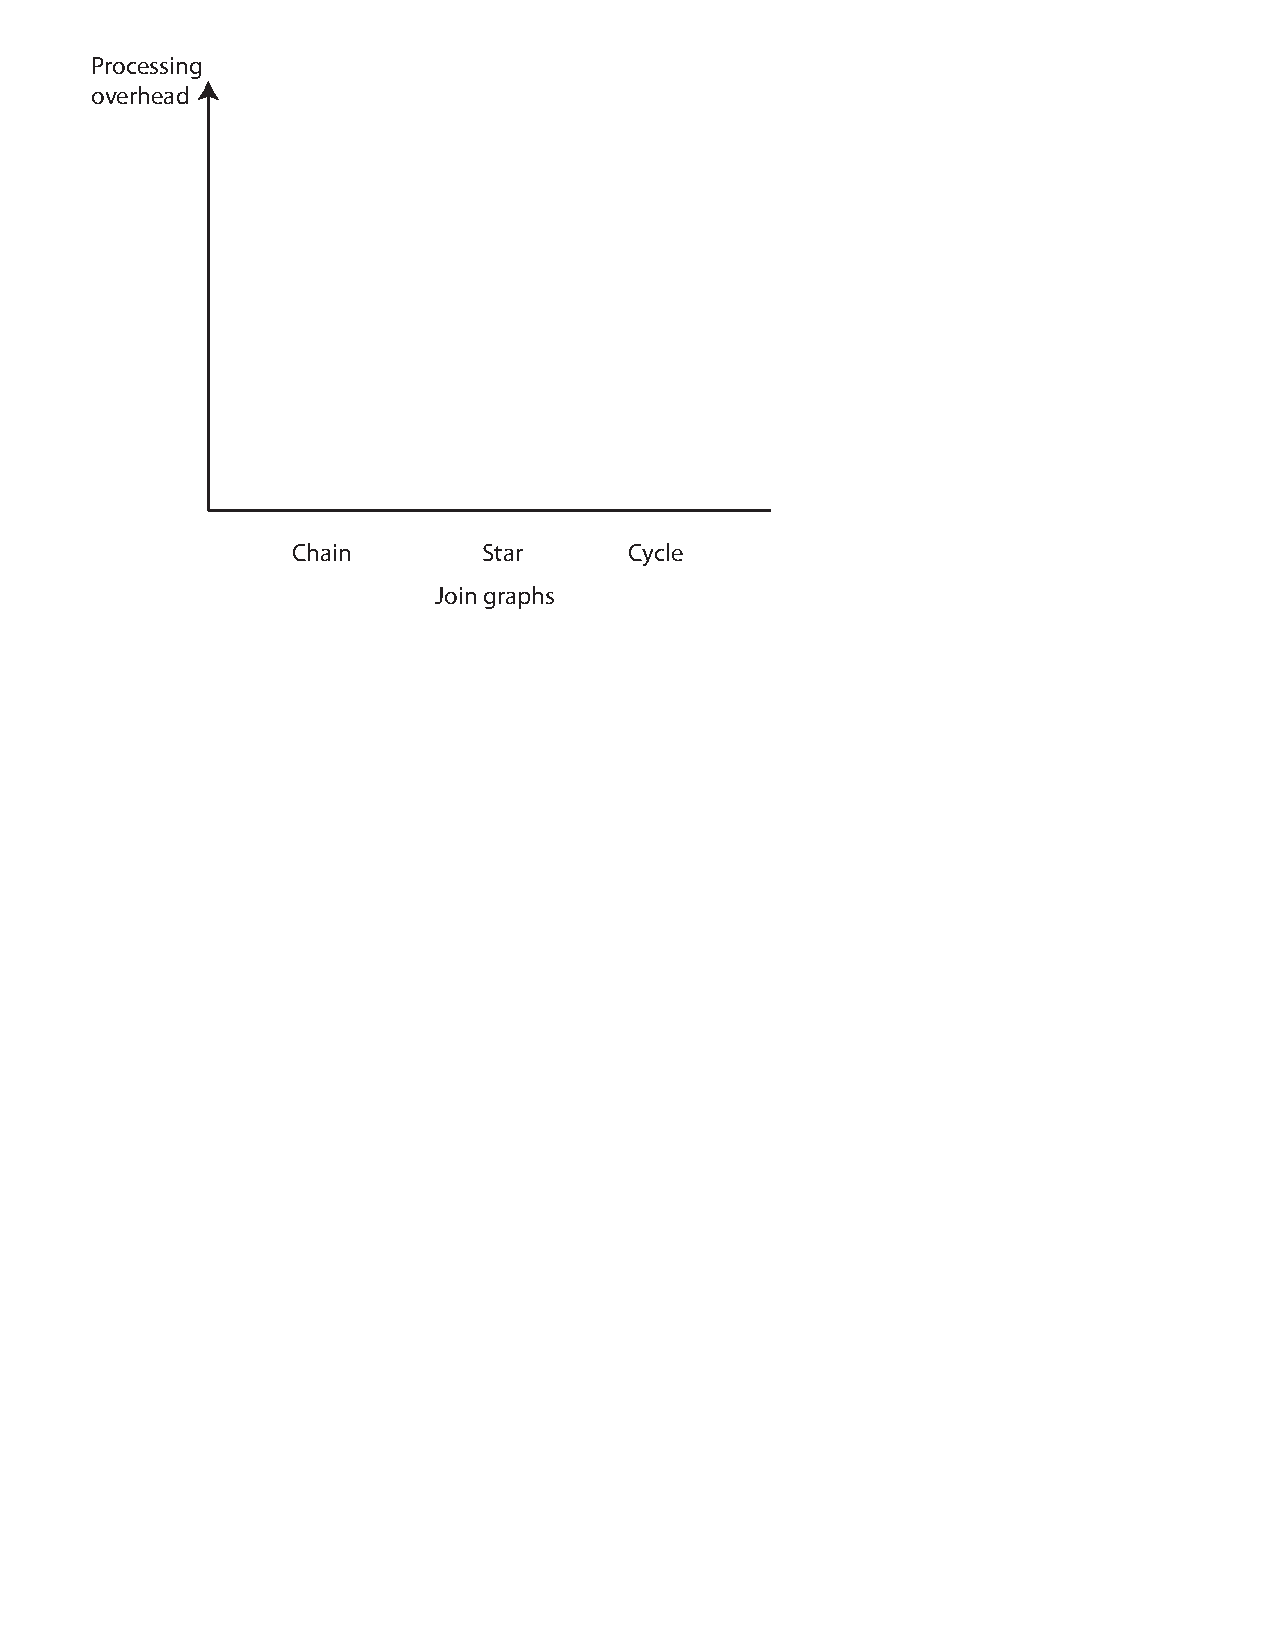
\includegraphics[scale=0.6]{figures/axes-jgraph.pdf}
\caption{Query processing overhead under varying join graph workloads for
recursive compilation and incremental view maintenance.}
\label{fig:overhead-workload-join}
\end{figure}

\subsubsection{Algorithmic Trading and Data Warehousing applications}

\begin{itemize}
\item Compare naive query processing and incremental view maintenance to full
DBToaster recursive compilation for real-world scenarios.
\end{itemize}

\begin{figure}
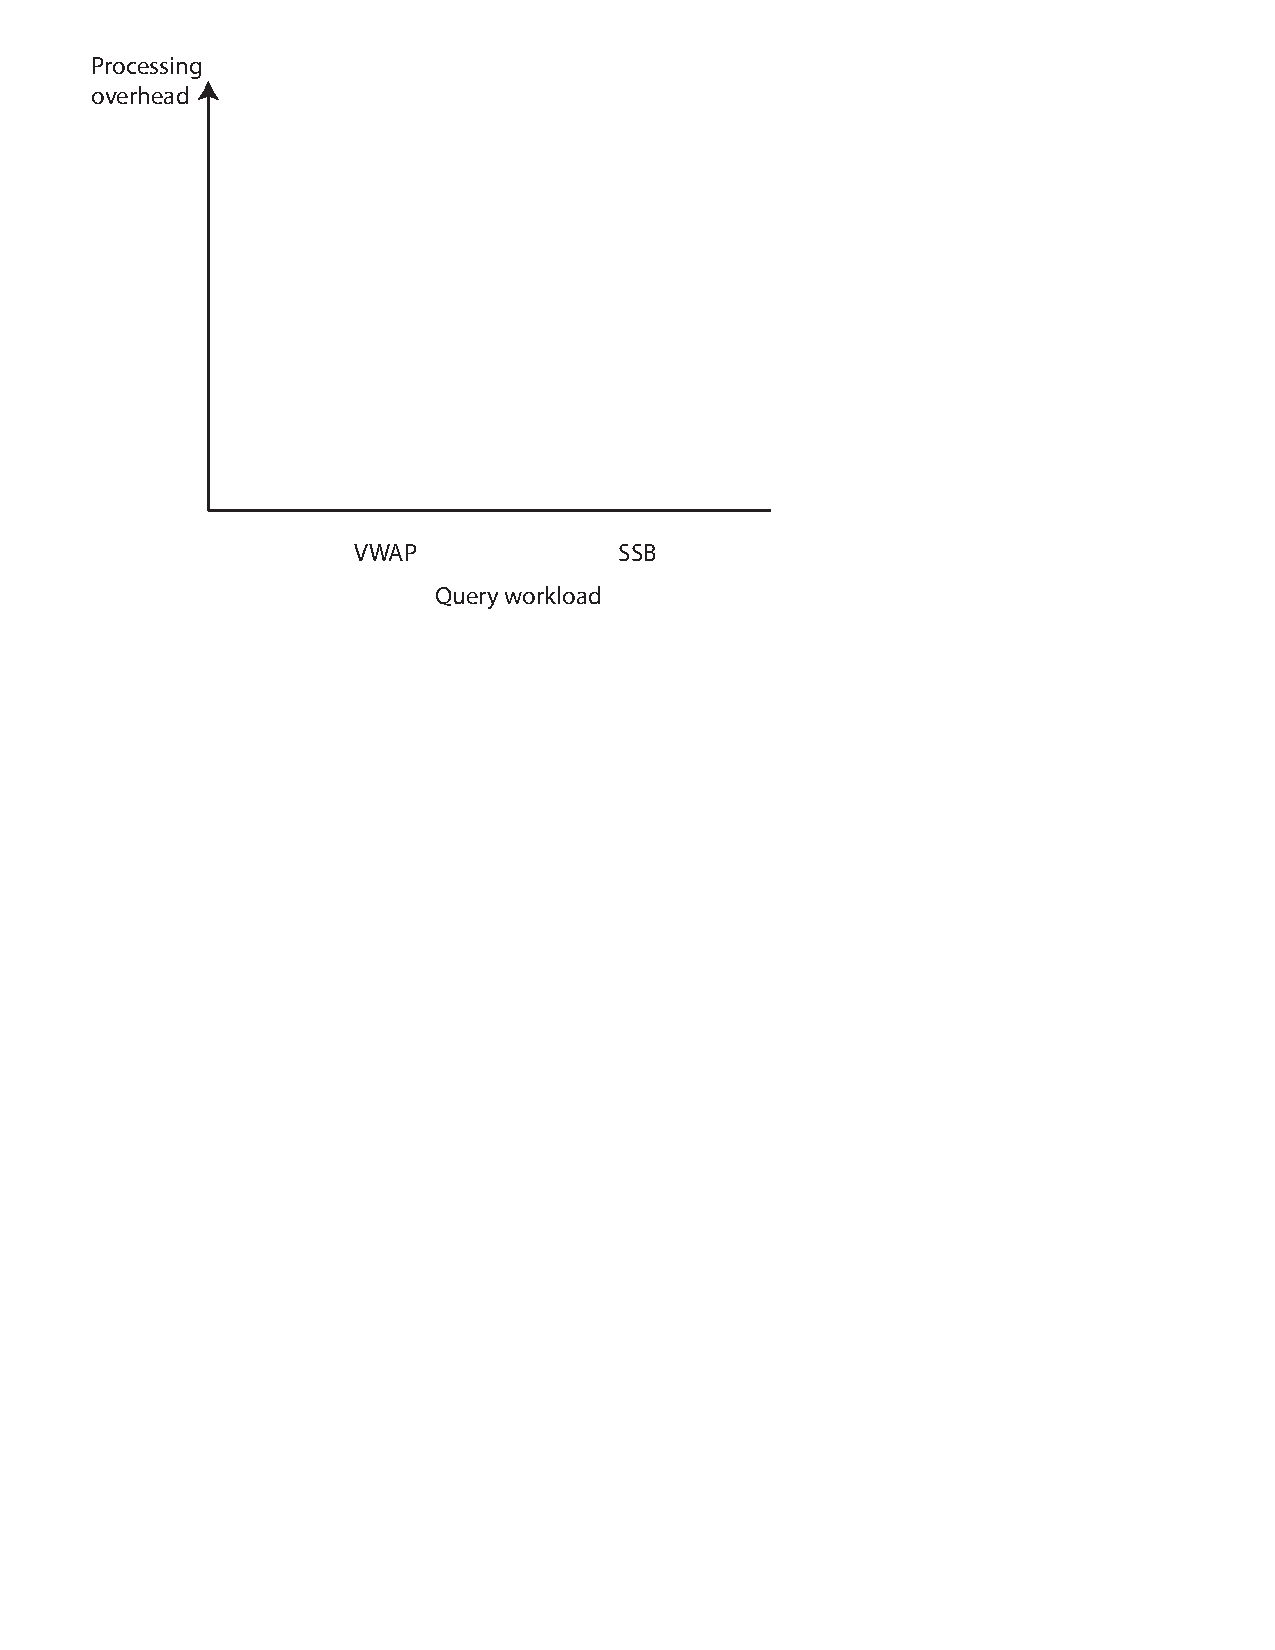
\includegraphics[scale=0.6]{figures/axes-query.pdf}
\caption{Query processing overheads for the VWAP and SSB queries, for naive
  query processing, incremental view maintenance and DBToaster.}
\label{fig:overhead-vwap-ssb}
\end{figure}
}


\comment{
\subsection{Memory Utilization}
\begin{itemize}
\item Measure total process memory usage over time, taking samples every $k$
  tuples (find a suitable value of $k$, perhaps 1000?).
\item Use the following formula to estimate a std::map$<>$ memory usage:
\begin{align*}
(sizeof(key) & + sizeof(value) + \\
& sizeof(rb\_tree\_node))*N\\
+ sizeof(rb\_tree)
\end{align*}

\item If time permits, use a custom allocator with an identifier for each map
assigned to use the allocator to track memory usage per map.

\item We have the following formulae for the number of maps created for k-way
joins with specific types of join graphs. These are derived by considering the
combinations of subgraphs of size $i$ (which constitute relations we can
aggregate), with $i = [1 \ldots k-1]$
    \begin{itemize}
    \item Chain: $\sum_{i=1}^{k}{i} = \frac{k(k+1)}{2}$
    \item Star: $(\sum_{i=1}^{k-1}{\binom{k-1}{i}}) + k $
    \item Cycle: $k*\sum_{i=1}^{k-1}{i} = \frac{k^2(k-1)}{2}$
    \end{itemize}

\item Predicted memory utilization:
    \begin{itemize}
    \item VWAP: mem(DBToaster) $>$ mem(VM) $>$ mem(naive) -- due to increased
    map usage, while still needing to maintain full domain. This changes if the base
    relation contains many duplicates, i.e. $|dom(P)| << |bids|$.
    \end{itemize}
\end{itemize}

\begin{figure}
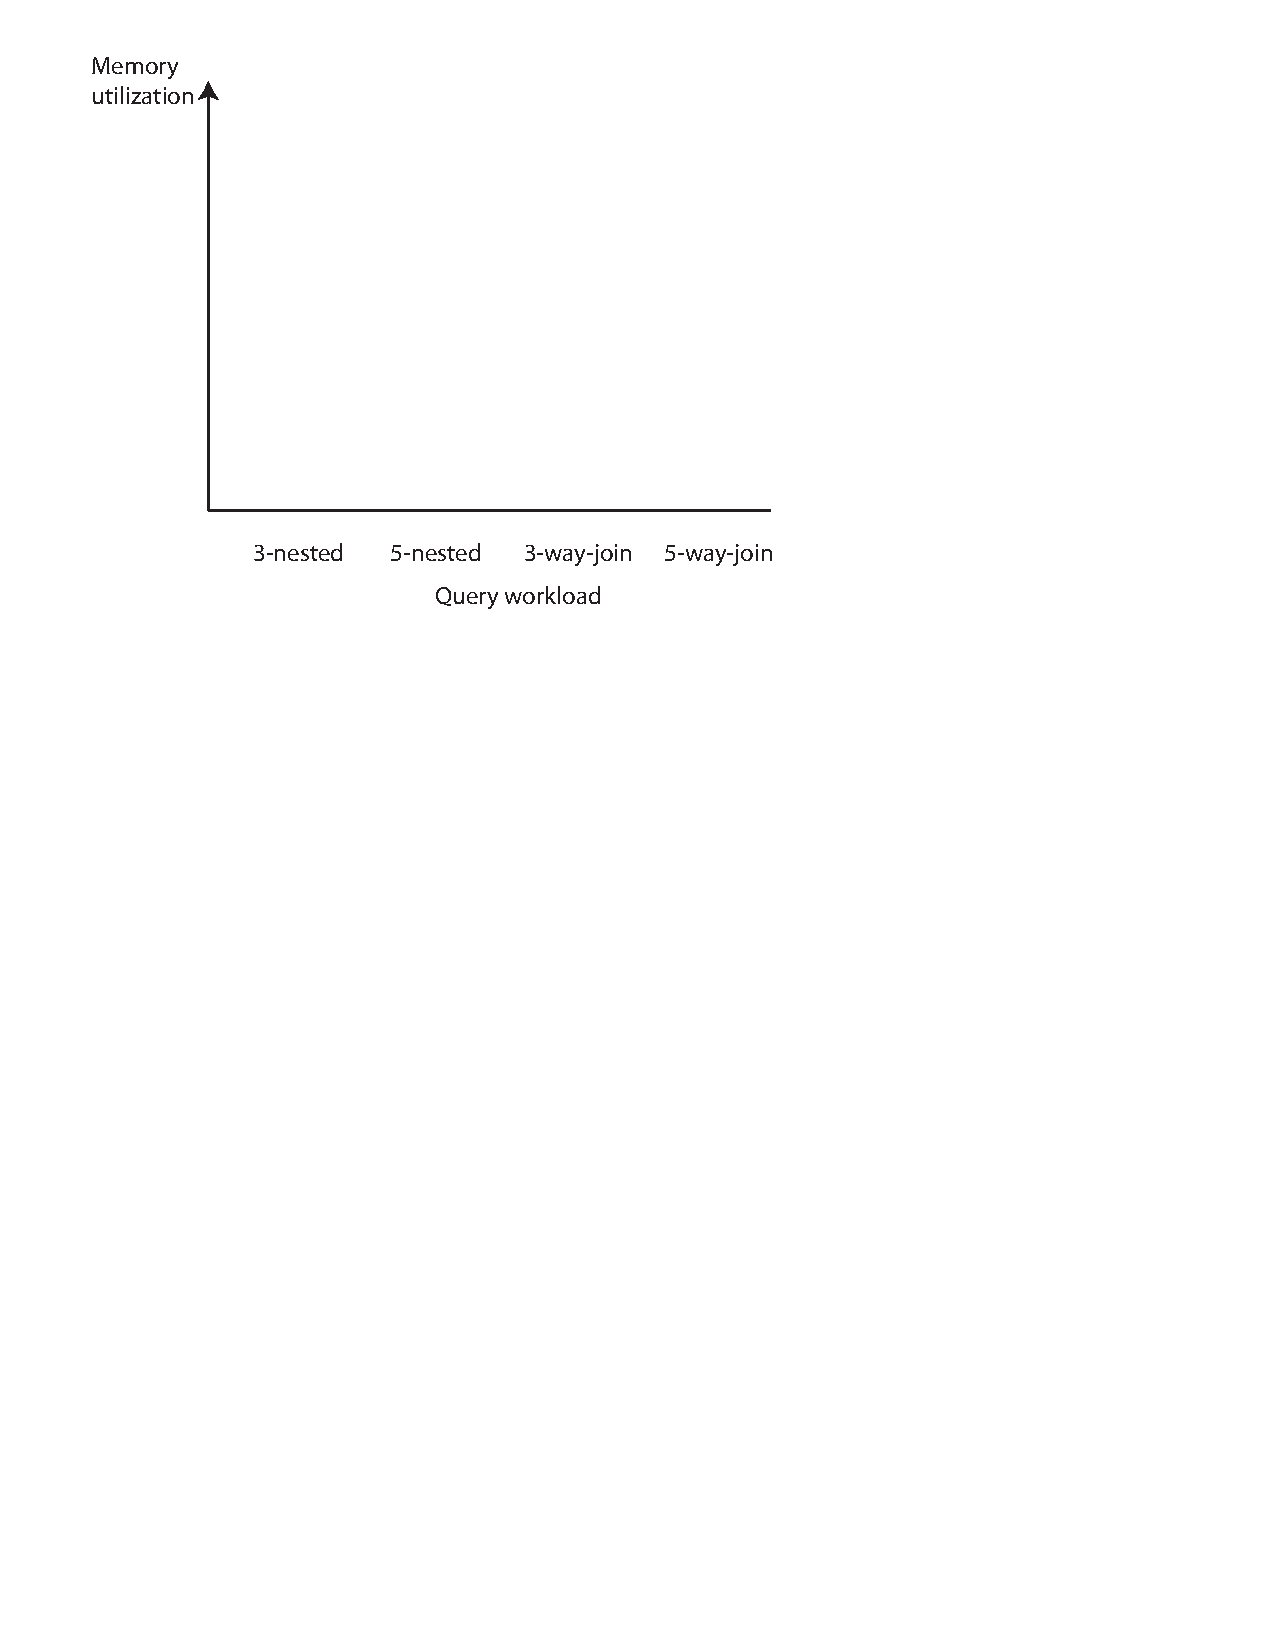
\includegraphics[scale=0.6]{figures/axes-memnjquery.pdf}
\caption{Memory utilization of the naive, incremental view maintenance, and
  DBToaster query processing techniques on nested and multiway join queries.}
\label{fig:memutil-njquery}
\end{figure}

\begin{figure}
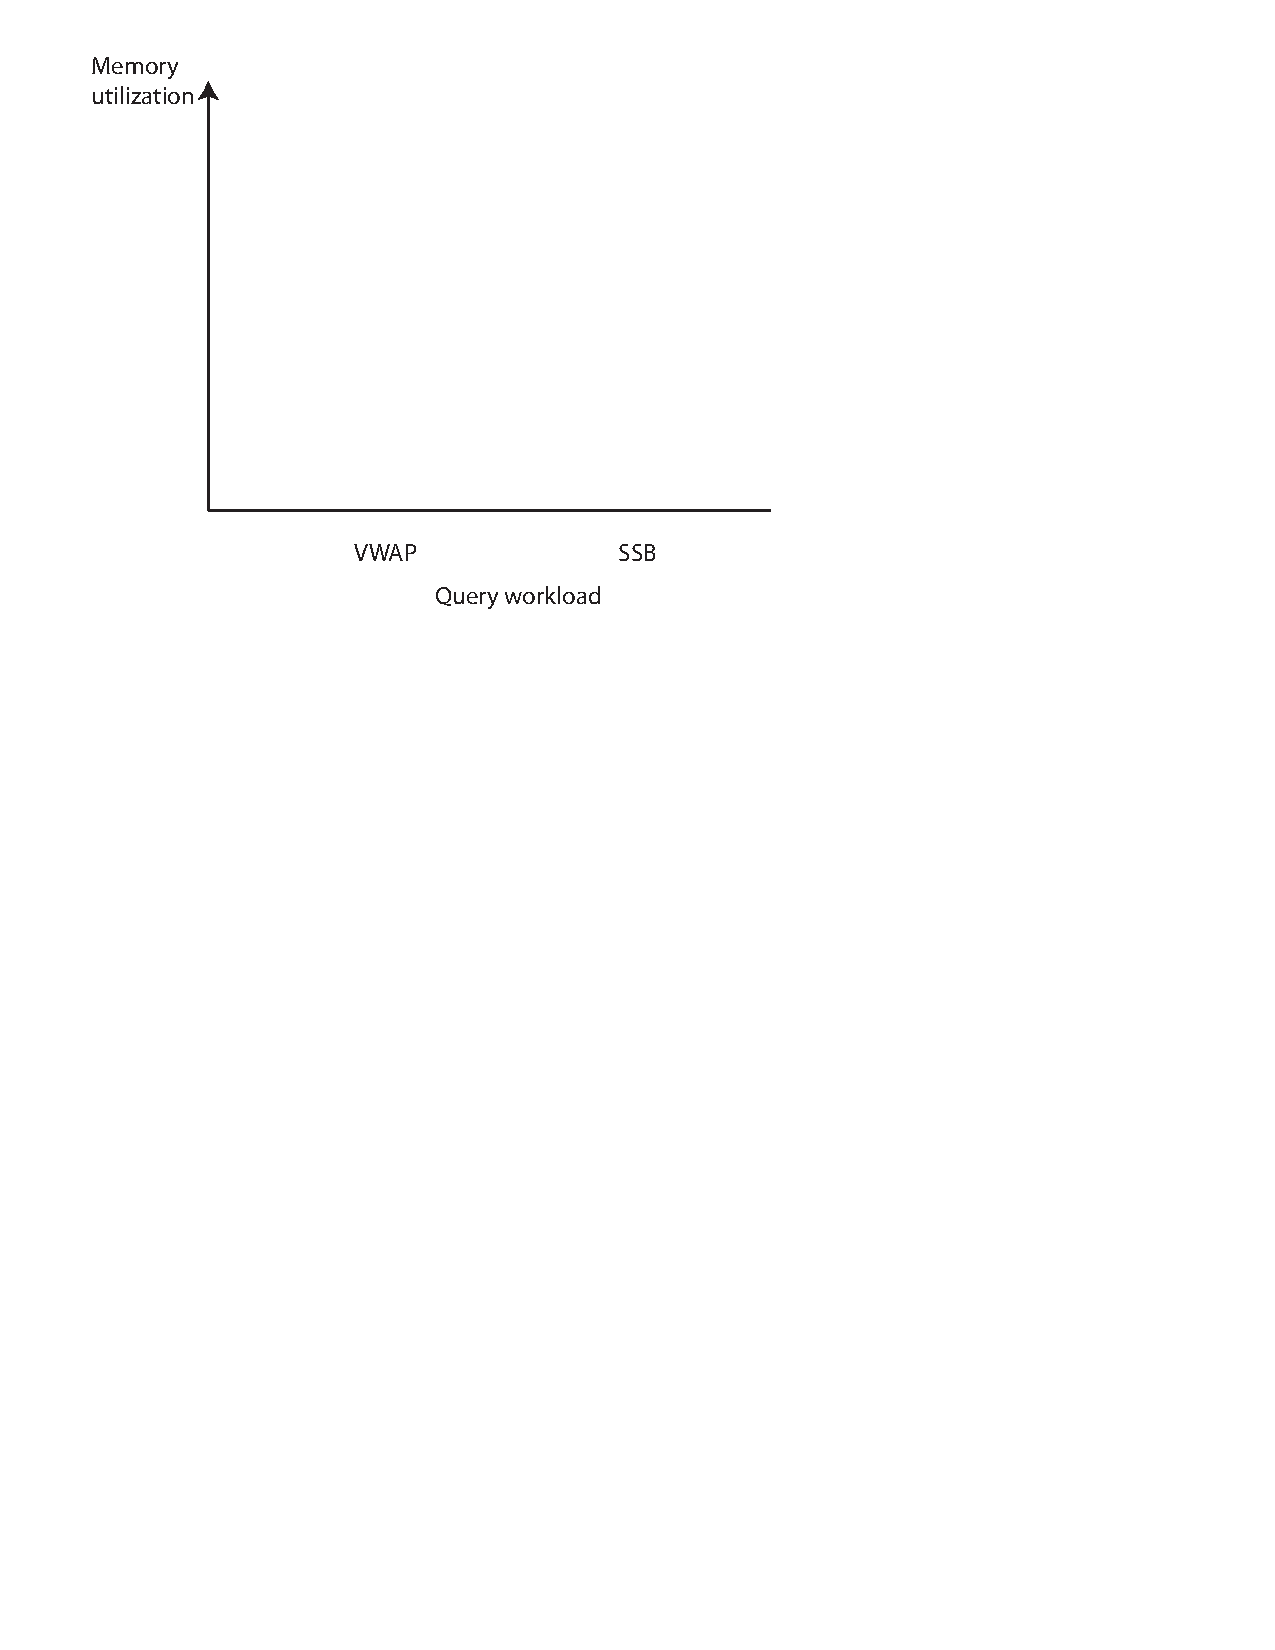
\includegraphics[scale=0.6]{figures/axes-memvsquery.pdf}
\caption{Memory utilization of the naive, incremental view maintenance, and
DBToaster query processing techniques for the VWAP and SSB queries.}
\label{fig:memutil-vsquery}
\end{figure}
}


\comment{
\subsection{DBMS Comparison}
\begin{itemize}
\item Compare DBToaster to Postgres, HSQLDB, Oracle (DBMS 'X'), Borealis,
  Streambase (DBMS 'Y').
\item Compare using four different techniques: repetitive processing, trigger
  processing, builtin view maintenance, and stream processing.
\item What about a column store, e.g. Vertica/MonetDB? This would only be
  possible under a repetitive QP technique (or does Vertica implement triggers?)
\end{itemize}

Notes on subquery processing in existing DBMS:
    \begin{itemize}
    \item Common techniques: subquery flattening, handling duplicates via a
    semijoin, replacing exists/any operators for single-row subqueries w/ early termination, etc.
    \item Apache Derby's subqueries:
    \url{http://db.apache.org/derby/docs/10.0/manuals/tuning/perf105.html#HDRSII-TRANSFORM-13699}
    \item Oracle's optimization of subqueries:
    \url{http://www.oracle.com/technology/products/bi/db/10g/pdf/twp_general_query_optimization_10gr2_0605.pdf}
    \item Oracle includes several implementations of semijoins, (hash-, sort-merge,
    etc.) allowing join optimization just as with regular joins.
    \item SQL Server subquery types:
    \url{http://technet.microsoft.com/en-us/library/ms175838.aspx}
    \item How does our naive nesting implementation compare with other DBMS's
    implementations of semijoins?
        \begin{itemize}
        \item We can ignore in/exists/any/all subqueries, and focus on scalar subqueries in predicates
        and select lists.
        \item Scalar aggregate subqueries must be evaluated fully, however, the subquery results for
        duplicate outer attributes can be cached and reused.
        \end{itemize}
    \end{itemize}

\subsubsection{Repetitive Processing}
\begin{itemize}
\item Check whether we can simply pass through queries to Postgres, DBMS 'X' and
  HSQLDB, or whether it's better to generate from map algebra due to specific
  SQL syntax for each DBMS.
\item Run experiment for repeating at various fractions of the dataset size,
  i.e. 10\%,20\%,...,100\%, where 100\% means running the query for every tuple.
\item Note other DBMS can exploit caching here significantly, while DBToaster
  currently does not perform caching, and is L1/L2 cache-agnostic.
\end{itemize}

\begin{figure}
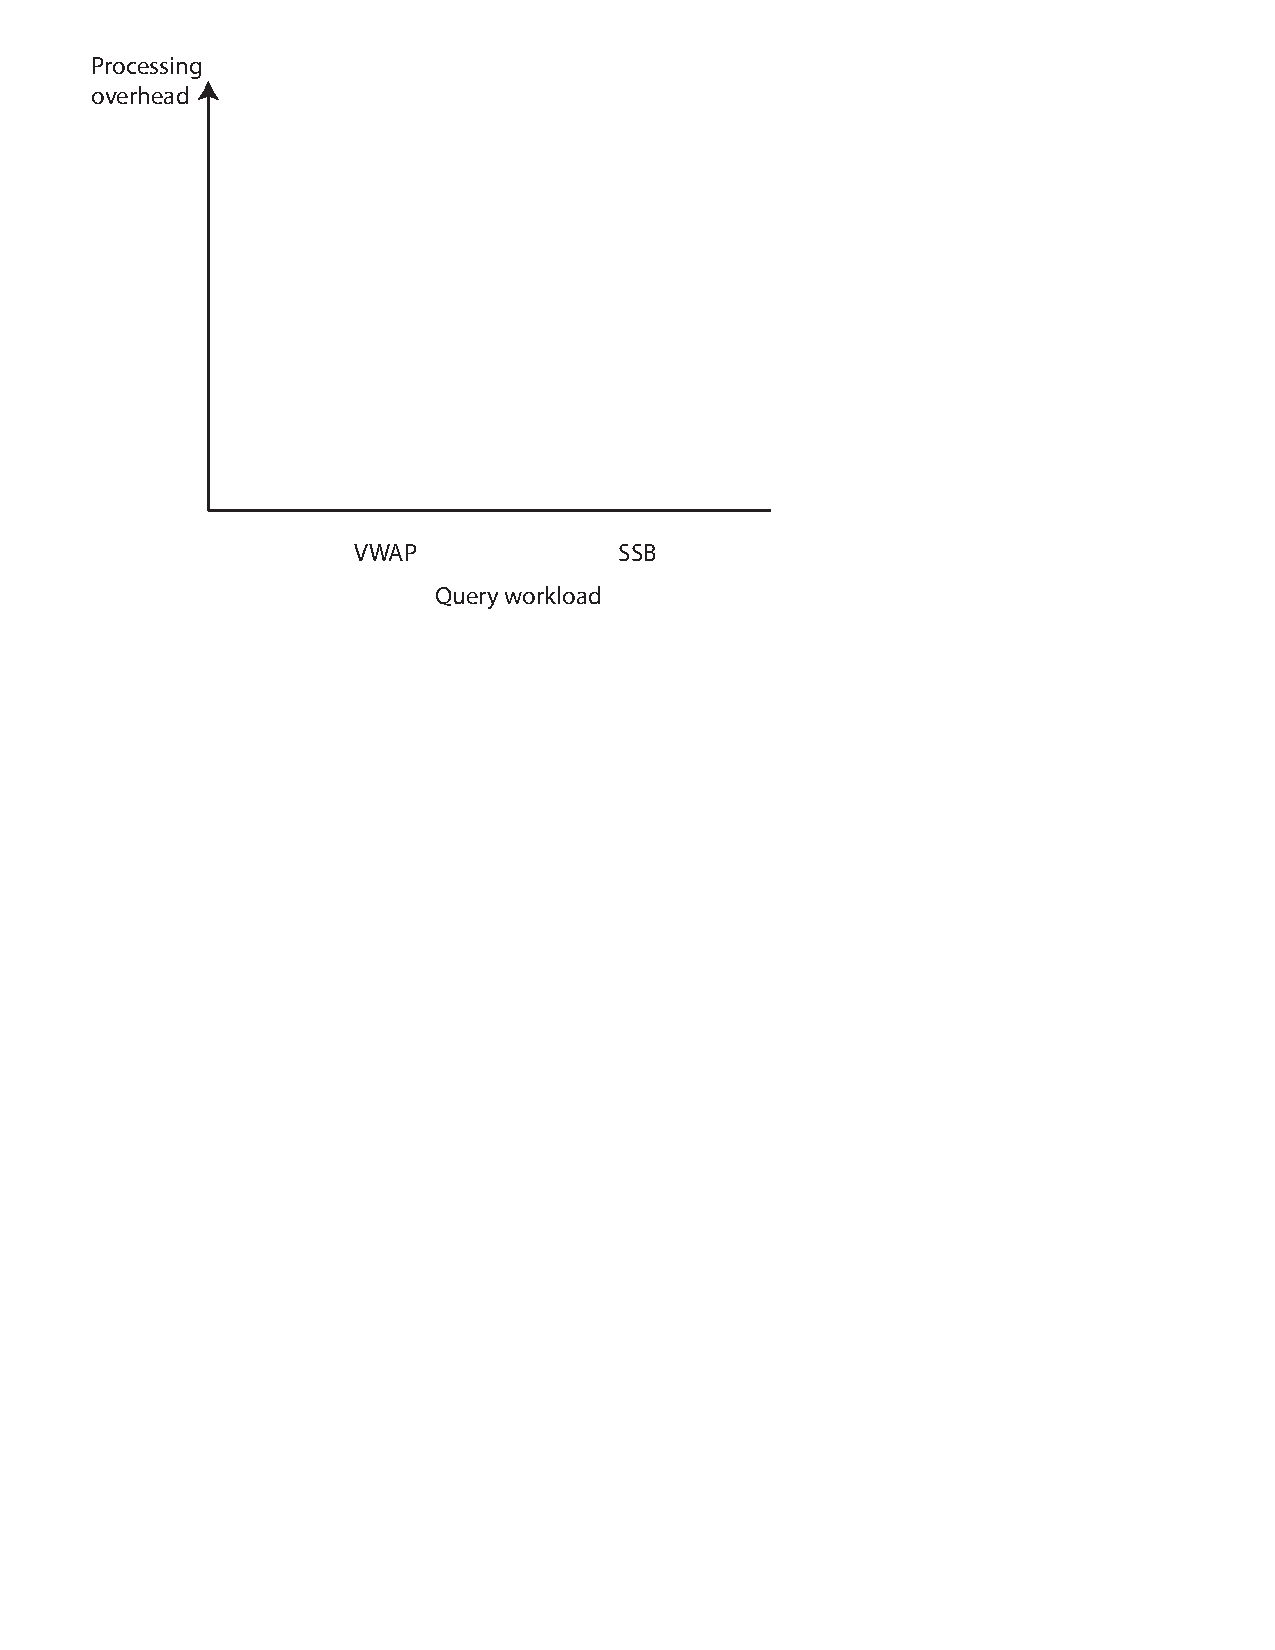
\includegraphics[scale=0.6]{figures/axes-repetitive.pdf}
\caption{Comparison of repetitive ad-hoc query processing of the VWAP and SSB
queries, in Postgres, DBMS 'X' and HSQLDB, to DBToaster's compiled query
processing.}
\label{fig:overhead-repetition}
\end{figure}

\subsubsection{Trigger-based processing}
\begin{itemize}
\item Generate trigger code from map algebra: use temporary tables as maps, and
  generate trigger code corresponding to each handler function.
\item HSQLDB only has Java-based triggers. Let's skip generating such Java-based
  triggers for now.
\item Postgres only allows row-based triggers to inspect tuple contents, DBMS
  'X' may allow access to the old and new tuple sets, allowing set-based
  triggering (like SQL Server).
\end{itemize}

\begin{figure}
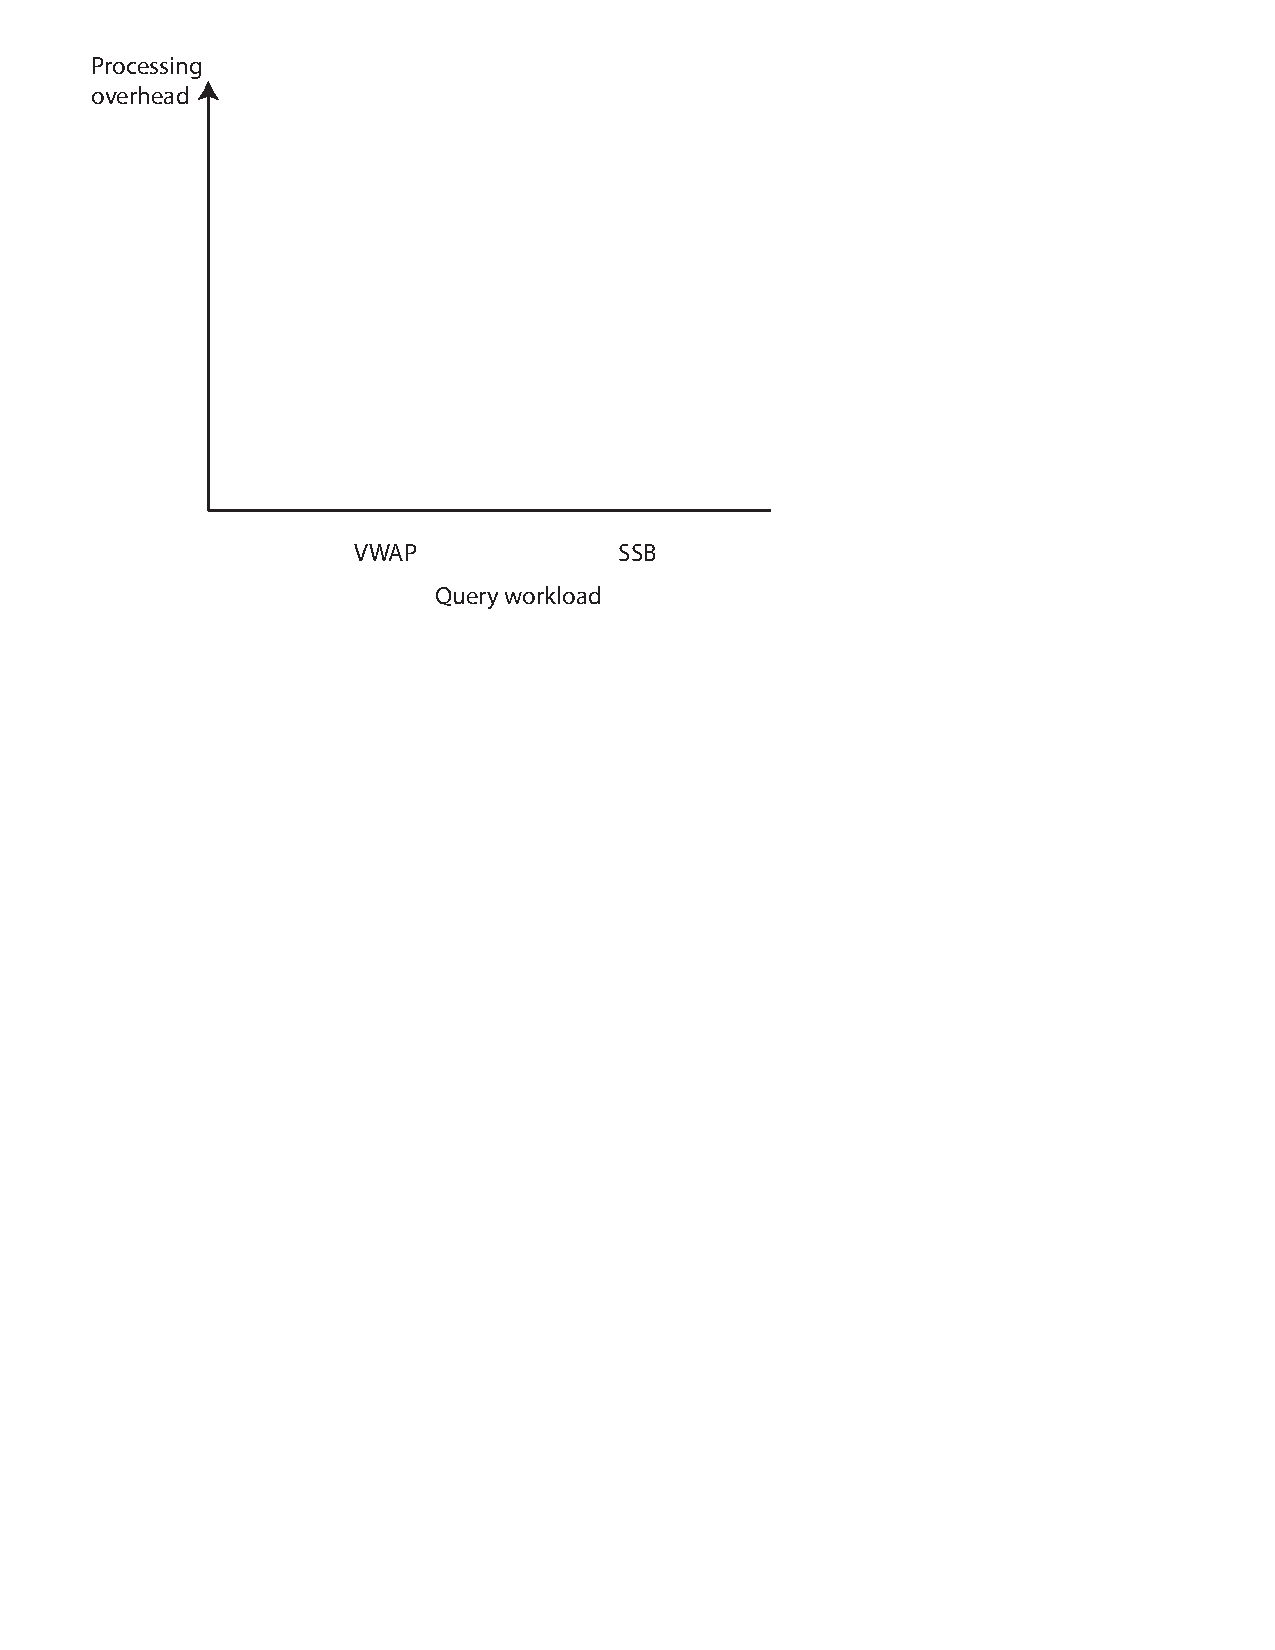
\includegraphics[scale=0.6]{figures/axes-triggers.pdf}
\caption{Comparison of trigger-based processing of the VWAP and SSB queries in
Postgres, DBMS 'X' and HSQLDB to DBToaster's compiled query processing}
\label{fig:overhead-trigger}
\end{figure}

\subsubsection{Materialized view maintenance}
\begin{itemize}
\item Pick a feasible query for view maintenance (perhaps TPCH/SSB queries...) since
  VWAP cannot be done via incremental view maintenance in DBMS 'X'.
\item Check if we can simply pass through user-specified query to DBMS 'X's create
  view DDL statement.
\end{itemize}

\begin{figure}
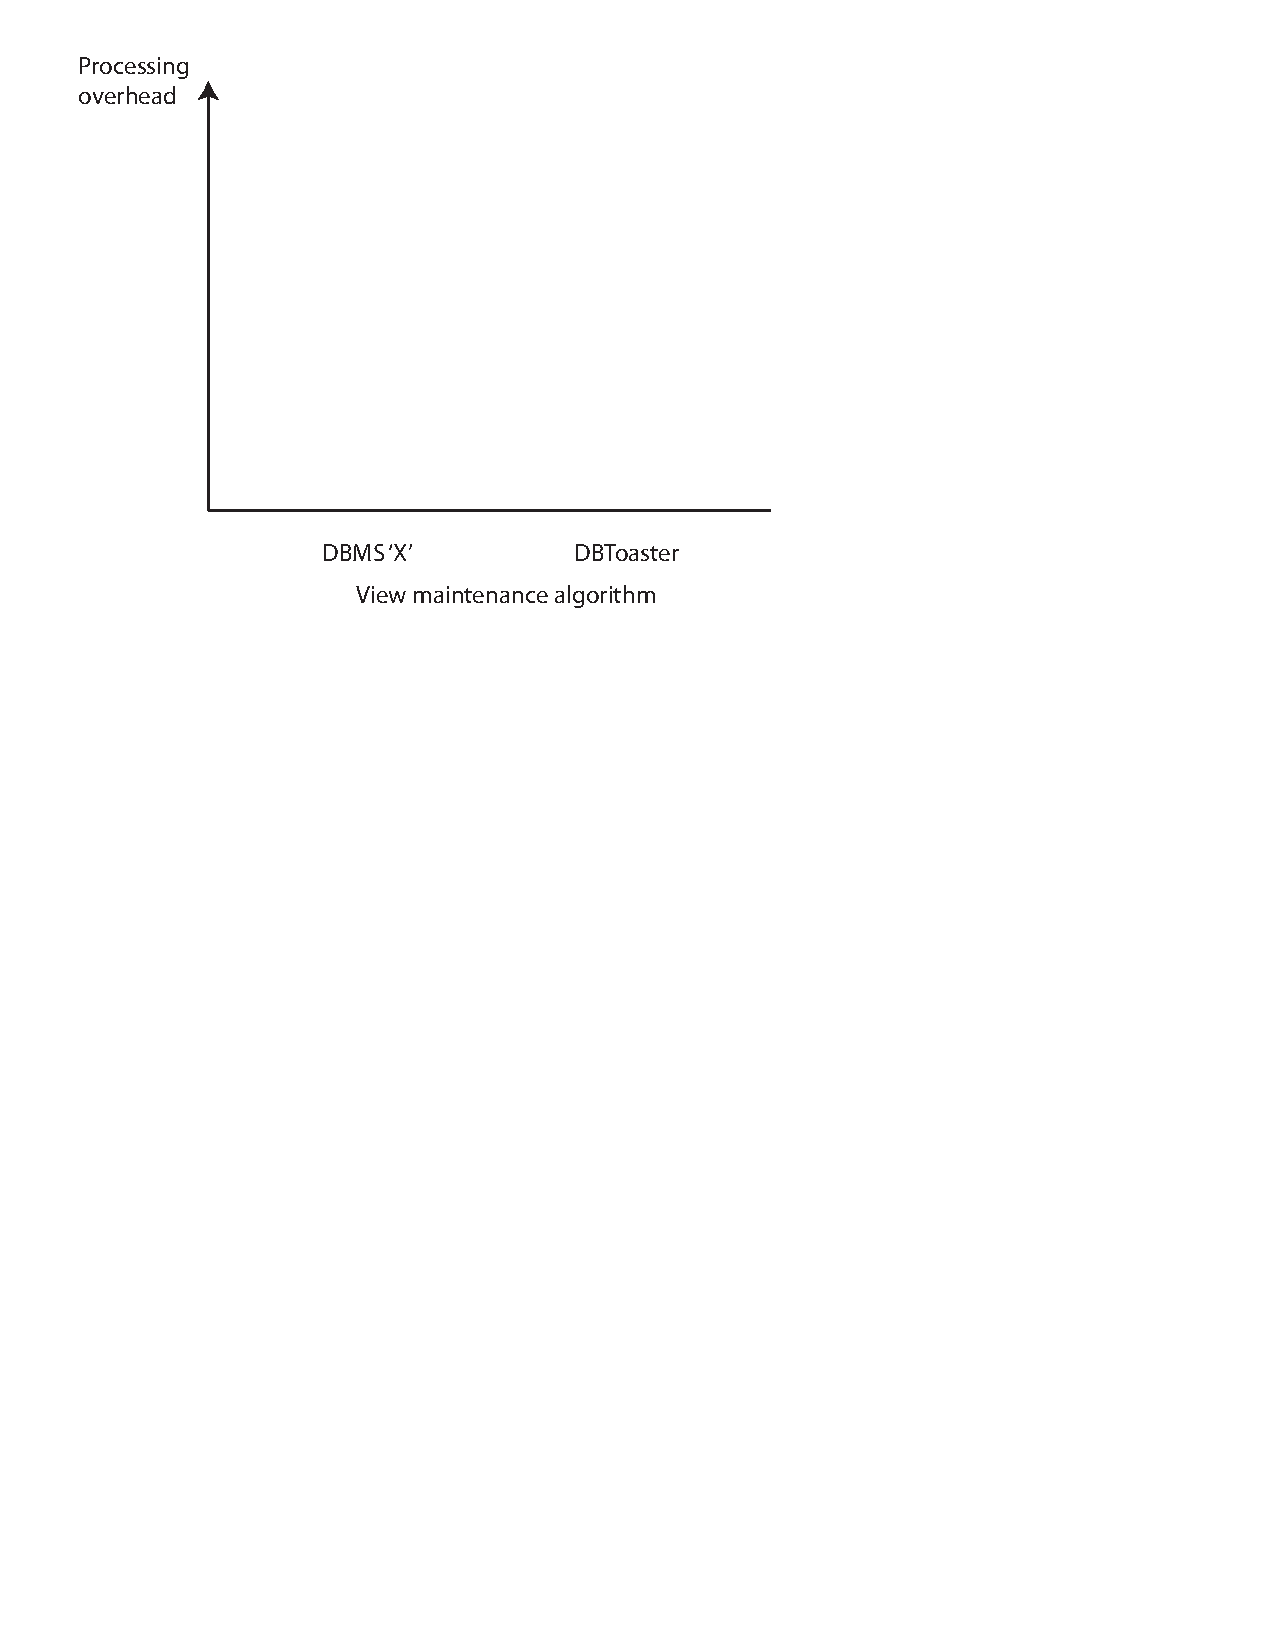
\includegraphics[scale=0.6]{figures/axes-views.pdf}
\caption{Comparison of view maintenance in DBMS 'X' to DBToaster's compiled query processing}
\label{fig:overhead-trigger}
\end{figure}

\subsubsection{Stream processing}
\begin{itemize}
\item Pick a feasible query for stream processing (i.e., pure stream processing
  query, perhaps Linear Road avg lav), that does not require the use of
  in-memory tables.
\item Compare both VWAP query and pure-stream query (i.e. with windowing
  expressed as a range predicate in DBToaster).
\item Generate Borealis XML representation and Streambase app XML representation
  directly from initial map algebra.
\end{itemize}

\begin{figure}
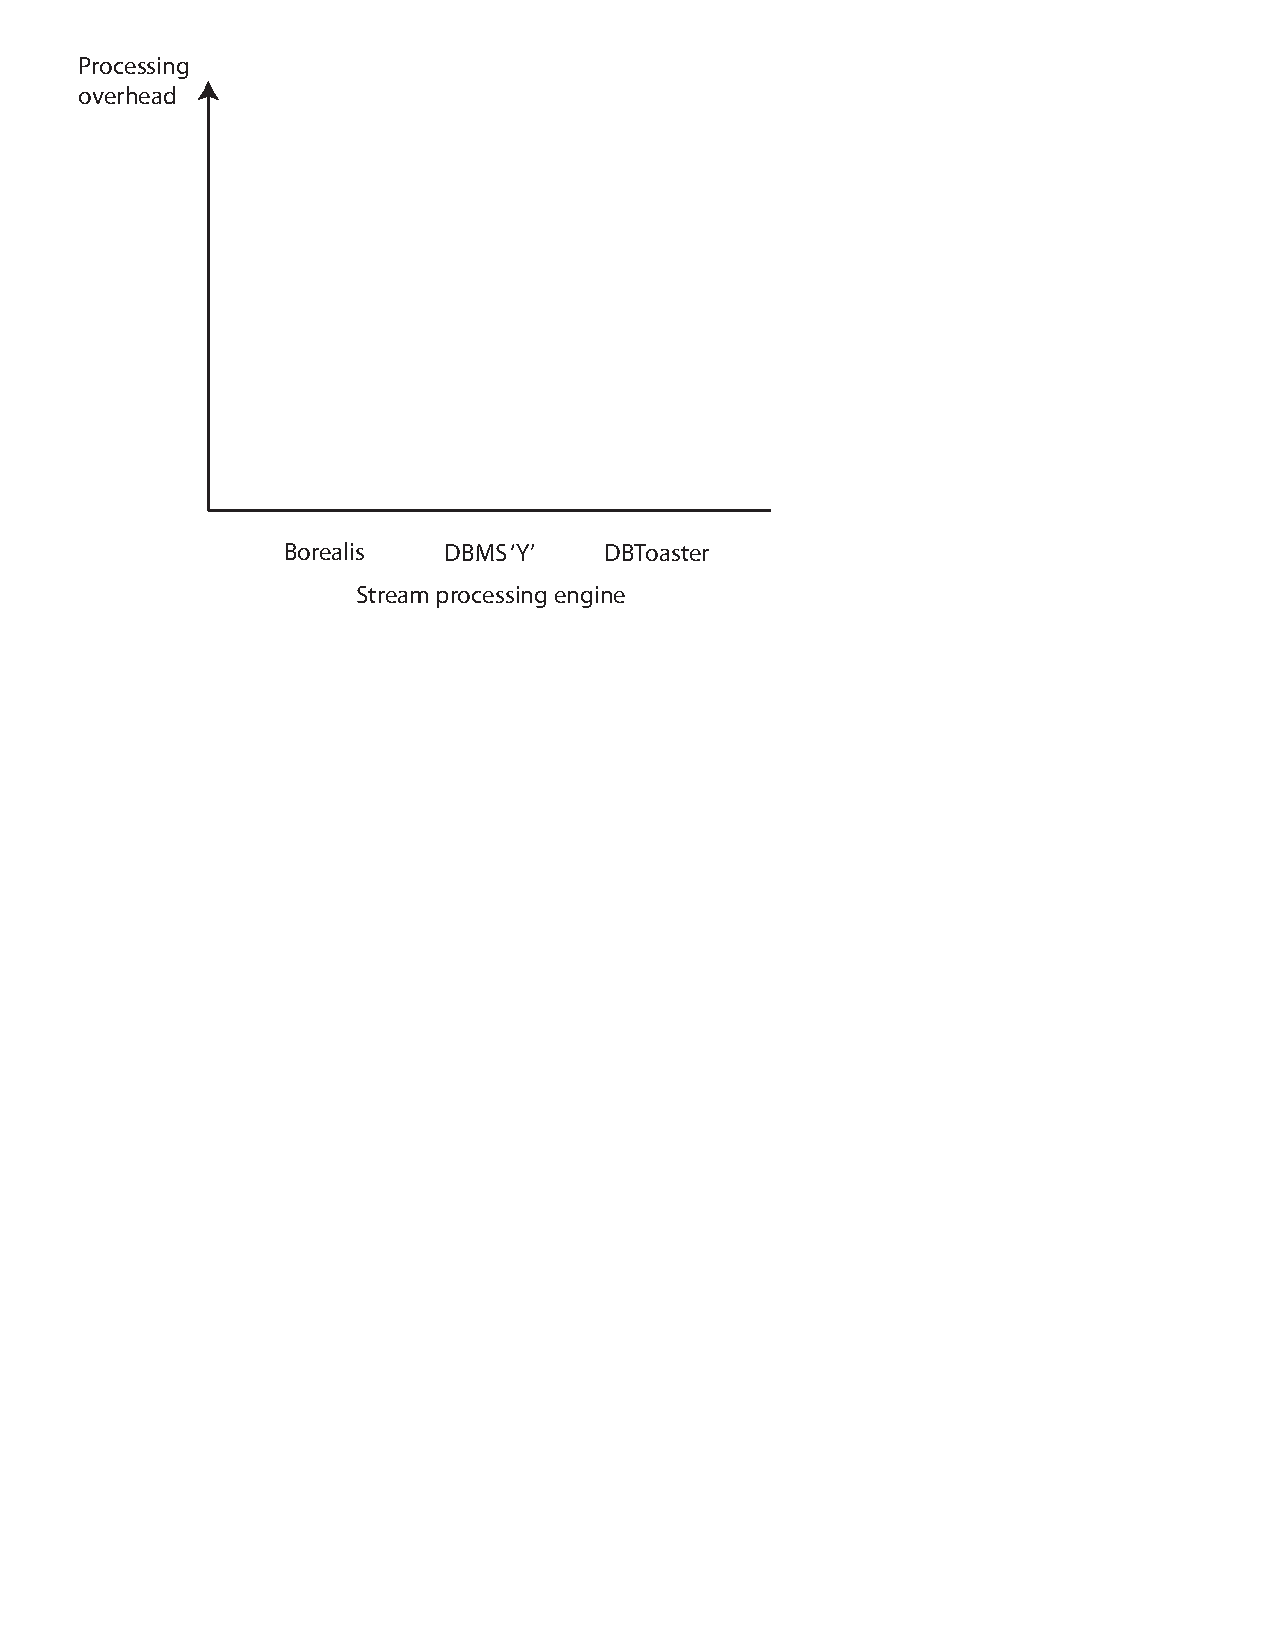
\includegraphics[scale=0.6]{figures/axes-streams.pdf}
\caption{Comparison of stream processing implementations of the XXX query, for
  Borealis and DBMS 'Y' to DBToaster's compiled query processing.}
\label{fig:overhead-stream}
\end{figure}
}